\documentclass{beamer}

\usepackage{color, colortbl}

\mode<presentation>
{
    %\usetheme{AnnArbor}
    %\usetheme{Antibes}
    %\usetheme{Bergen}
    %\usetheme{Berkeley}
    %\usetheme{Berlin}
    %\usetheme{Boadilla}
    %\usetheme{CambridgeUS}
    %\usetheme{Copenhagen}
    %\usetheme{Darmstadt}
    %\usetheme{Dresden}
    %\usetheme{Frankfurt}
    %\usetheme{Goettingen}
    %\usetheme{Hannover}
    %\usetheme{Ilmenau}
    %\usetheme{JuanLesPins}
    %\usetheme{Luebeck}
    \usetheme{Madrid}
    %\usetheme{Malmoe}
    %\usetheme{Marburg}
    %\usetheme{Montpellier}
    %\usetheme{PaloAlto}
    %\usetheme{Rochester}
    %\usetheme{Singapore}            % maybe
    %\usetheme{Szeged}
    %\usetheme{Warsaw}
    %\setbeamercovered{transparent}
    \usecolortheme{seahorse}
}

\setbeamertemplate{footline}
{
  \leavevmode%
  \hbox{%
  \begin{beamercolorbox}[wd=.2\paperwidth,ht=2.25ex,dp=1ex,center]{author in head/foot}%
	  \usebeamerfont{author in head/foot}Martin Hru\v{s}ka
  \end{beamercolorbox}%
  \begin{beamercolorbox}[wd=.7\paperwidth,ht=2.25ex,dp=1ex,center]{title in head/foot}%
    \usebeamerfont{title in head/foot}\insertshorttitle
  \end{beamercolorbox}}%
  \begin{beamercolorbox}[wd=.1\paperwidth,ht=2.25ex,dp=1ex,center]{date in head/foot}
            \insertframenumber{} / \inserttotalframenumber 
        \end{beamercolorbox}%
  \vskip0pt%
}

\setbeamertemplate{itemize item}[square]
\setbeamertemplate{itemize subitem}[triangle]
\setbeamertemplate{itemize subsubitem}[circle]
% \setbeamertemplate{enumerate item}[square]
\setbeamertemplate{section in toc}[square]
\setbeamertemplate{navigation symbols}{}

\newenvironment{figure*}%
{\begin{figure}}
{\end{figure}}

\usepackage{adjustbox}
\usepackage{comment}
\usepackage{ucs}
\usepackage[utf8x]{inputenc}
%\usepackage{palatino}
\usepackage{color}
\usepackage{graphicx}
%\usepackage{alltt}
\usepackage{tikz}
\usepackage{subcaption}
%\usepackage{MnSymbol}
%\usepackage{wasysym}
\usepackage[nofillcomment,noend,linesnumbered,noline,oldcommands]{algorithm2e}
\usetikzlibrary{calc,matrix,backgrounds,fit,shapes,arrows}

\usetikzlibrary{arrows}
\usetikzlibrary{backgrounds}
\usetikzlibrary{calc}
\usetikzlibrary{fit}
\usetikzlibrary{decorations}
\usetikzlibrary{decorations.pathmorphing}
\usetikzlibrary{decorations.pathreplacing}

\newcommand{\hlbl}[1]{\textcolor{blue}{#1}}
\newcommand{\hlgr}[1]{\textcolor{olive!50!green}{#1}}
\newcommand{\hlrd}[1]{\textcolor{red}{#1}}
\newcommand{\hlye}[1]{\textcolor{magenta}{#1}}
\newcommand{\hcol}[1]{yellow!20!orange!20}
\newcommand{\ucol}[1]{red!50}
\newcommand{\scol}[1]{blue!40}

\newcommand{\todo}[1]{\hlbl{[TODO: #1]}} 
\newcommand{\nt}[1]{\hlgr{[NOTE: #1]}} 

\newcommand{\heap}{h}
\newcommand{\heaps}{\mathcal{H}}
\newcommand{\partrel}{\approx}
\newcommand{\ta}{\mathit{TA}}
\newcommand{\langof}[1]{\mathcal{L}(#1)}


% for the table
\newcommand{\safe}[0]{safe}
\newcommand{\unsafe}[0]{error}

\newcommand{\mytree}{%
  \begin{tikzpicture}
  [
    scale=0.6,
    transform shape
  ]
    \path[use as bounding box] (-2.4mm,0mm) rectangle (2.4mm,5mm);
    %\draw (0mm,0mm) -- (0mm,5mm);
    \filldraw (0mm,5mm) -- (-2mm,3mm) -- (0mm,4mm) -- (0mm,3.5mm) -- (-2mm,1.5mm) --
    (0mm,2.5mm) -- (0mm,0.5mm) -- (0mm,2.5mm) -- (2mm,1.5mm) -- (0mm,3.5mm) --
    (0mm,4mm) -- (2mm,3mm) -- cycle;
  \end{tikzpicture}%
}

\newcommand{\dls}{
  \begin{tikzpicture}
  [
    baseline,
    anchor=base
  ]
    \node[draw,fill=blue!30,rectangle] {DLS};
  \end{tikzpicture}
}

\newcommand{\greensmile}{\textcolor{olive!50!green}{\textbf{\smiley}}}
\newcommand{\redfrown}{\textcolor{red}{\textbf{\frownie}}}

\renewcommand*{\thefootnote}{\fnsymbol{footnote}}

% Subtitle all from paper title
\title{
 Counterexample Validation and Interpolation-Based
Refinement for Forest Automata}
\author[
  Hol\'{i}k \and 
  \textbf{\hlbl{Hru\v{s}ka}} \and
  Leng\'{a}l \and
  Rogalewicz \and
  Vojnar~~~~~]
{
  Luk\'{a}\v{s} Hol\'{i}k \and 
  \hlbl{\textbf{ Martin Hru\v{s}ka}} \and
  Ond\v{r}ej~Leng\'{a}l \and
  Adam~Rogalewicz\\ \and
  Tom\'{a}\v{s}~Vojnar}

\institute[BUT]{Brno University of Technology, Czech Republic\\[6mm]
@VMCAI'17, Paris}


\date{January 16, 2017}

\begin{document}

%REMOVE
%\includeonlyframes{current}

%*******************************************************************************
\begin{frame}[plain]
  \titlepage
\end{frame}
%*******************************************************************************

%*******************************************************************************
\begin{frame}
  \frametitle{Introduction}
  \begin{itemize}
	  \item Shape analysis using \hlbl{Forest Automata (FA)}
		  (tuples of tree automata)
		  \begin{itemize}
			\item Reasoning about programs with dynamic linked data structures
				(tree structures, nested structures, \hlbl{structures with properties\,---\,contribution of this work})
			\item Notoriously \hlbl{difficult}: infinite sets of complex graphs
			\item Verifying properties such as \hlbl{reachability of~an error state} and \hlbl{memory safety}\,---\,absence of~null pointer dereference,
			  memory leak, or invalid free
	  \end{itemize}
	%  \item Analysis of programs with \hlbl{complex} dynamic data structures
	%  \begin{itemize}
	%	  \item tree structures
	%	  \item nested structures (linked lists with nested linked lists)
	%	  \item \hlbl{structures with properties (contribution of this work)}
	%  \end{itemize}
	% \item \hlbl{Verifying properties} such as
	%	  reachability of~an error state and absence of~null pointer dereference,
	%	  memory leak, or invalid free
	  \pause
	  	  \item Implemented in the \hlbl{Forester} tool\,---\,analysis of C programs
	  \item \hlgr{Advantages}
	   \begin{itemize}
		 \item Generality of the approach
		 \item Powerful and precise (thanks to refinement) abstraction
		 \item Scalability
	   \end{itemize}

  \end{itemize}
\end{frame}
%*******************************************************************************

%*******************************************************************************
\begin{frame}
  \frametitle{An Overview of Verification Method}
   \begin{itemize}
	   \item Based on \hlbl{Abstract Regular Tree Model Checking (ARTMC) and CEGAR} 
		\begin{itemize}
			\item Sets of program configurations are represented by automata
	%		\item Starts with an automaton representing initial configuration
	%		\item Applying a transducer modelling behaviour of system until a fixpoint is reached
	%		\item Employs \hlbl{abstraction} over automata to overapproximate sets of~reachable configurations
	%			after each application of transducer
	%		\item Make intersection of fixpoint automaton with automaton representing bad behaviour and
	%			checks emptiness of its language
		\end{itemize}
	%	\pause
	%   \item Employs \hlbl{CEGAR} to refine abstraction over automata
	%	   \begin{itemize}
	%		    \item Forward run with abstraction
	%		    \item Backward run for validation of counterexample (CE)
	%			\item Refinement of abstraction to avoid spurious CE
	%	   \end{itemize}
	%	\pause
	   \vspace{0.2cm}
	   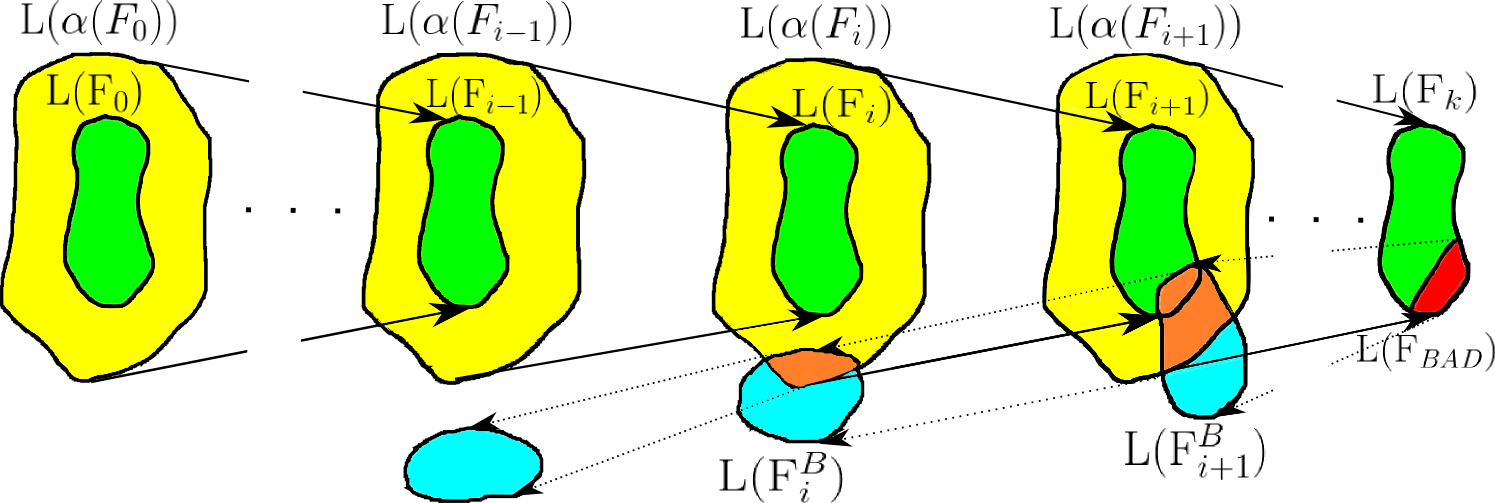
\includegraphics[scale=0.26]{artmc.png}
		   \pause
	   \item CEGAR applied to ARTMC, but not to FA
		   based shape analysis $\rightarrow$ \hlrd{contribution} of this work
  \end{itemize}
\end{frame}
%*******************************************************************************

%*******************************************************************************
\begin{frame}
\frametitle{Outline of the Talk}

	\begin{enumerate}
		\item Example
		\item Forest Automata based Shape Analysis
		\item Evaluation and Conclusion
	\end{enumerate}

\end{frame}

%*******************************************************************************

%*******************************************************************************
\begin{frame}
% \begin{frame}[label=current]
  \frametitle{Example\,---\,Forward Run no. 1}
  \begin{overlayarea}{7cm}{6.5cm}
      \only<1>{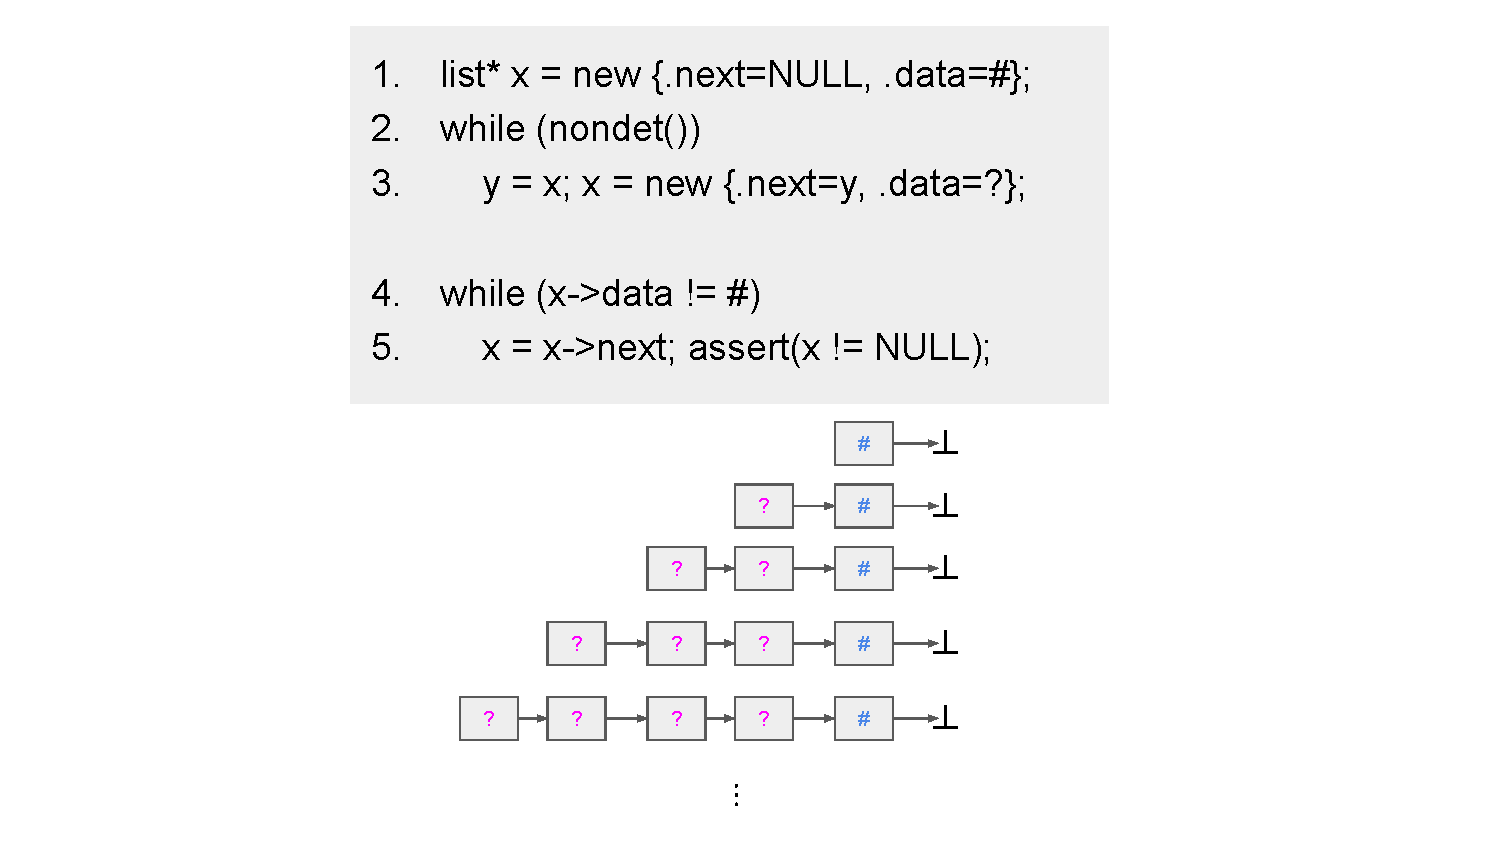
\includegraphics[scale=0.5]{ex/vmcai_1.pdf}}
      \only<2>{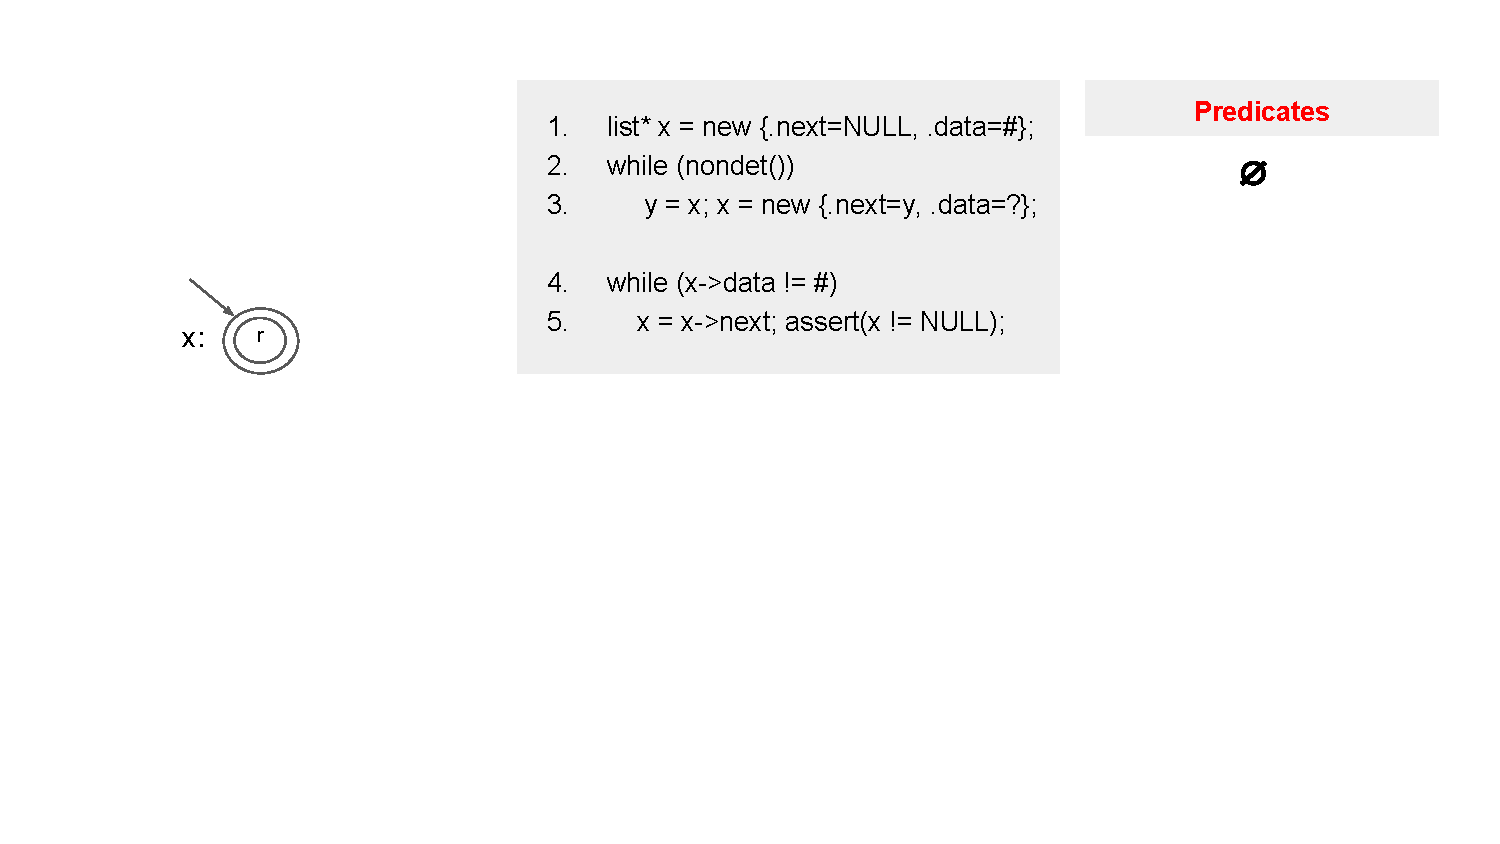
\includegraphics[scale=0.5]{ex/vmcai_2.pdf}}
      \only<3>{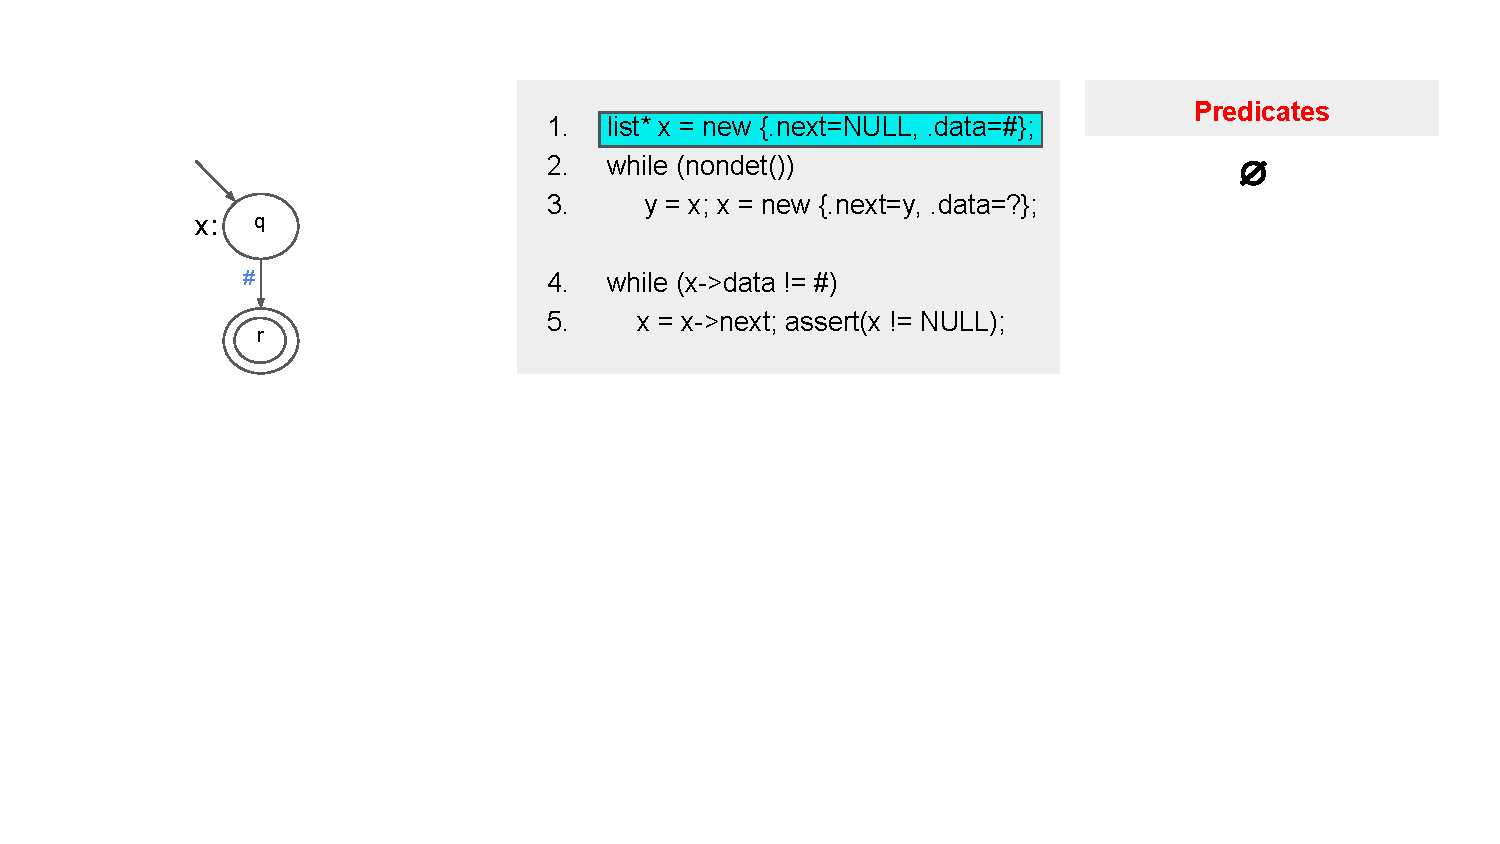
\includegraphics[scale=0.5]{ex/vmcai_3.pdf}}
      \only<4>{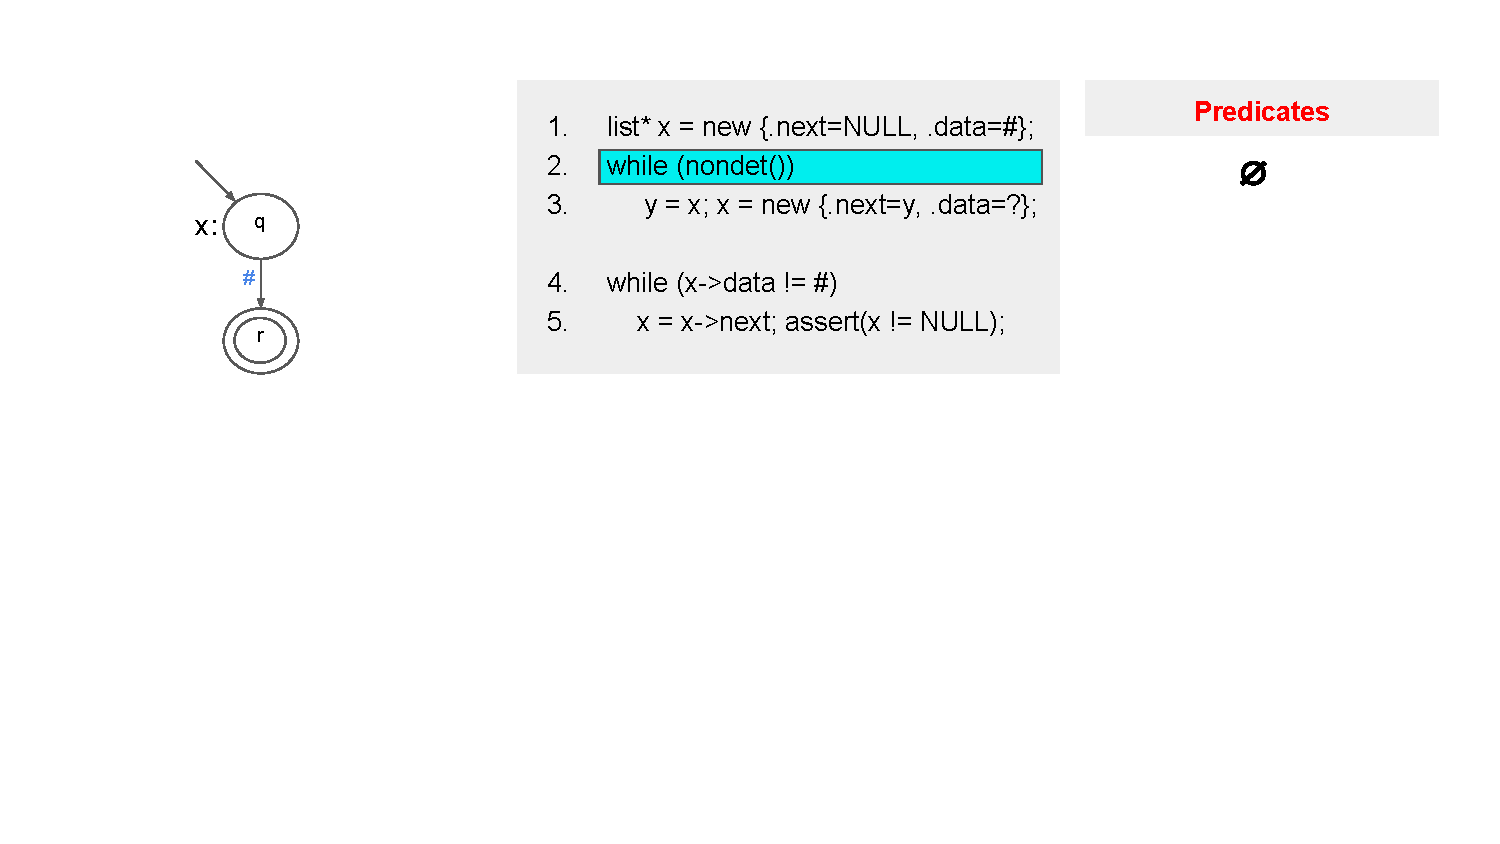
\includegraphics[scale=0.5]{ex/vmcai_4.pdf}}
      \only<5>{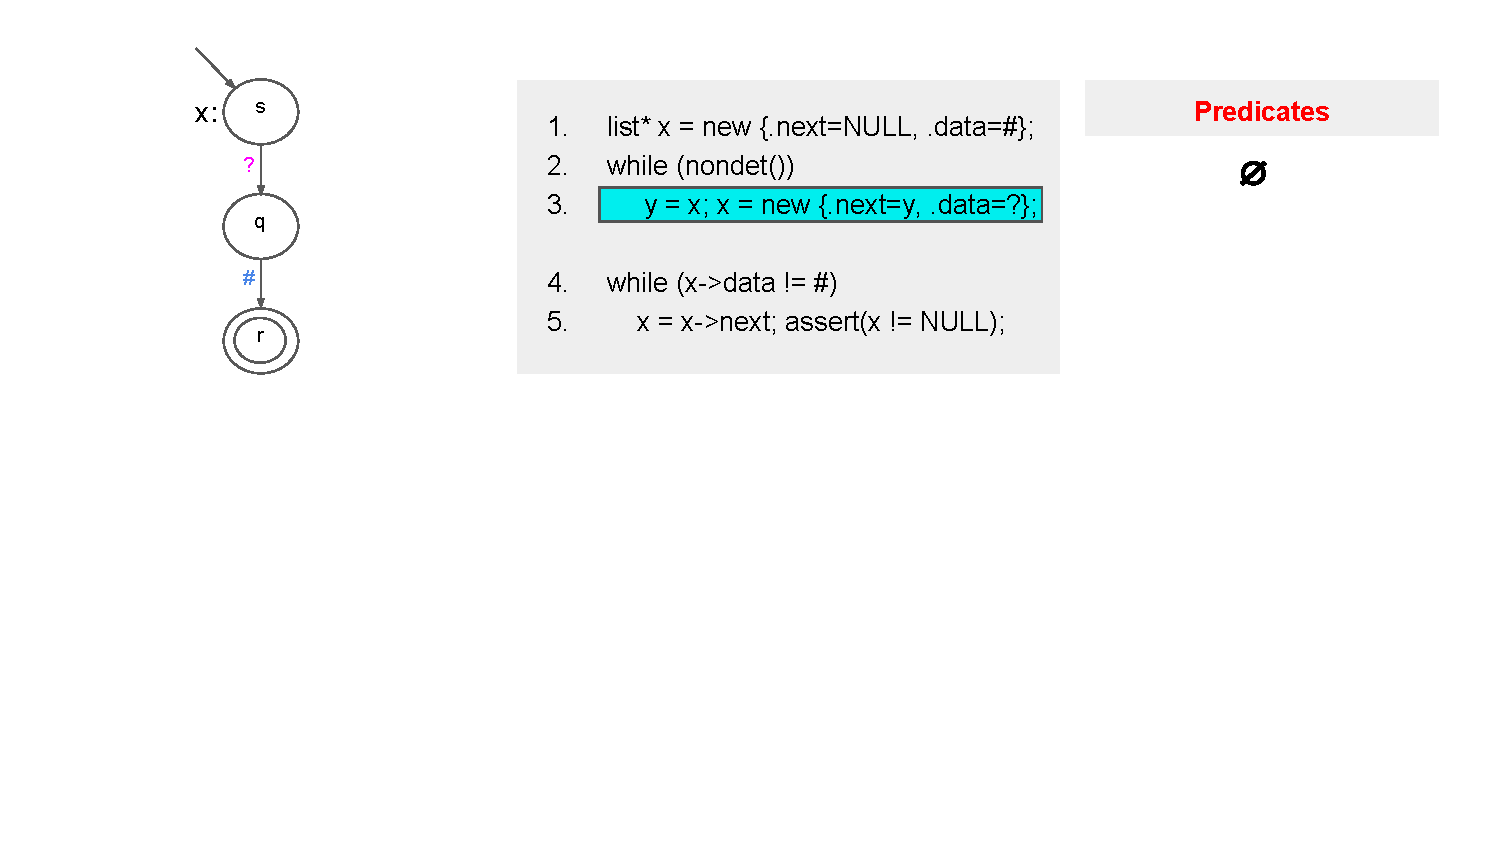
\includegraphics[scale=0.5]{ex/vmcai_5.pdf}}
      \only<6>{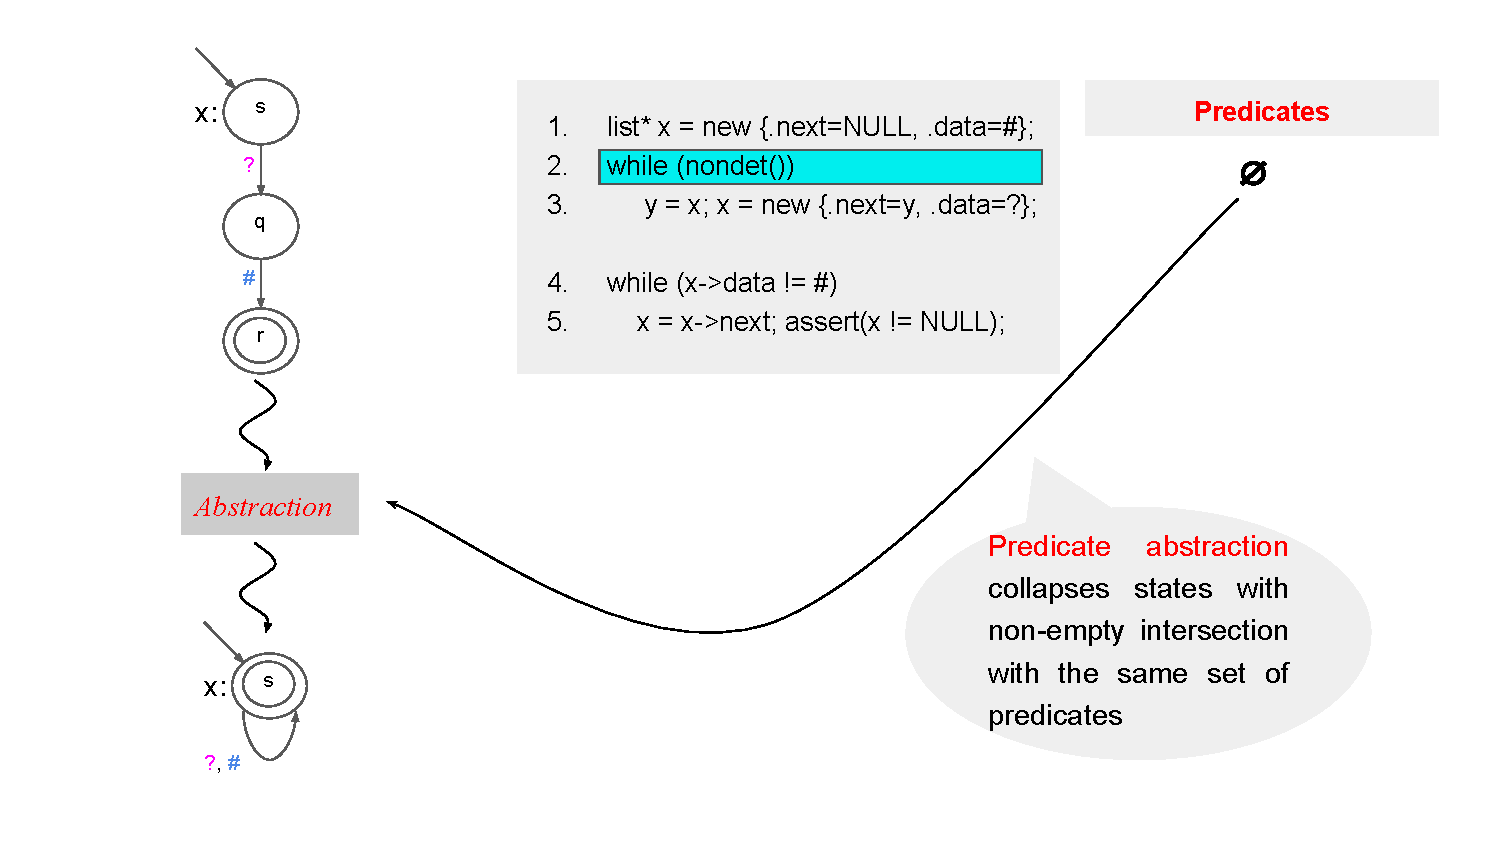
\includegraphics[scale=0.5]{ex/vmcai_6.pdf}}
      \only<7>{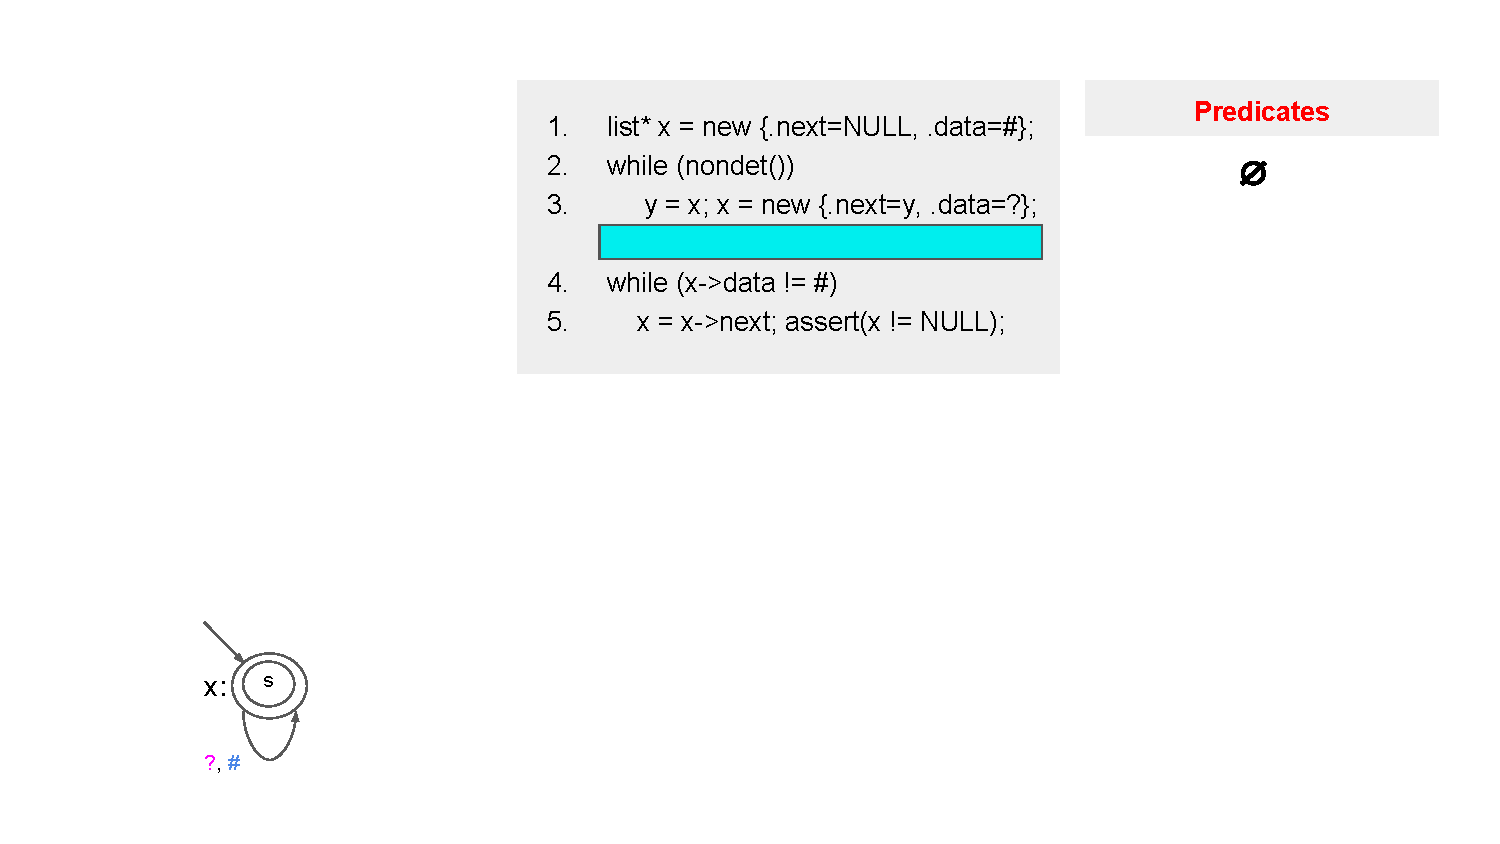
\includegraphics[scale=0.5]{ex/vmcai_7.pdf}}
      \only<8>{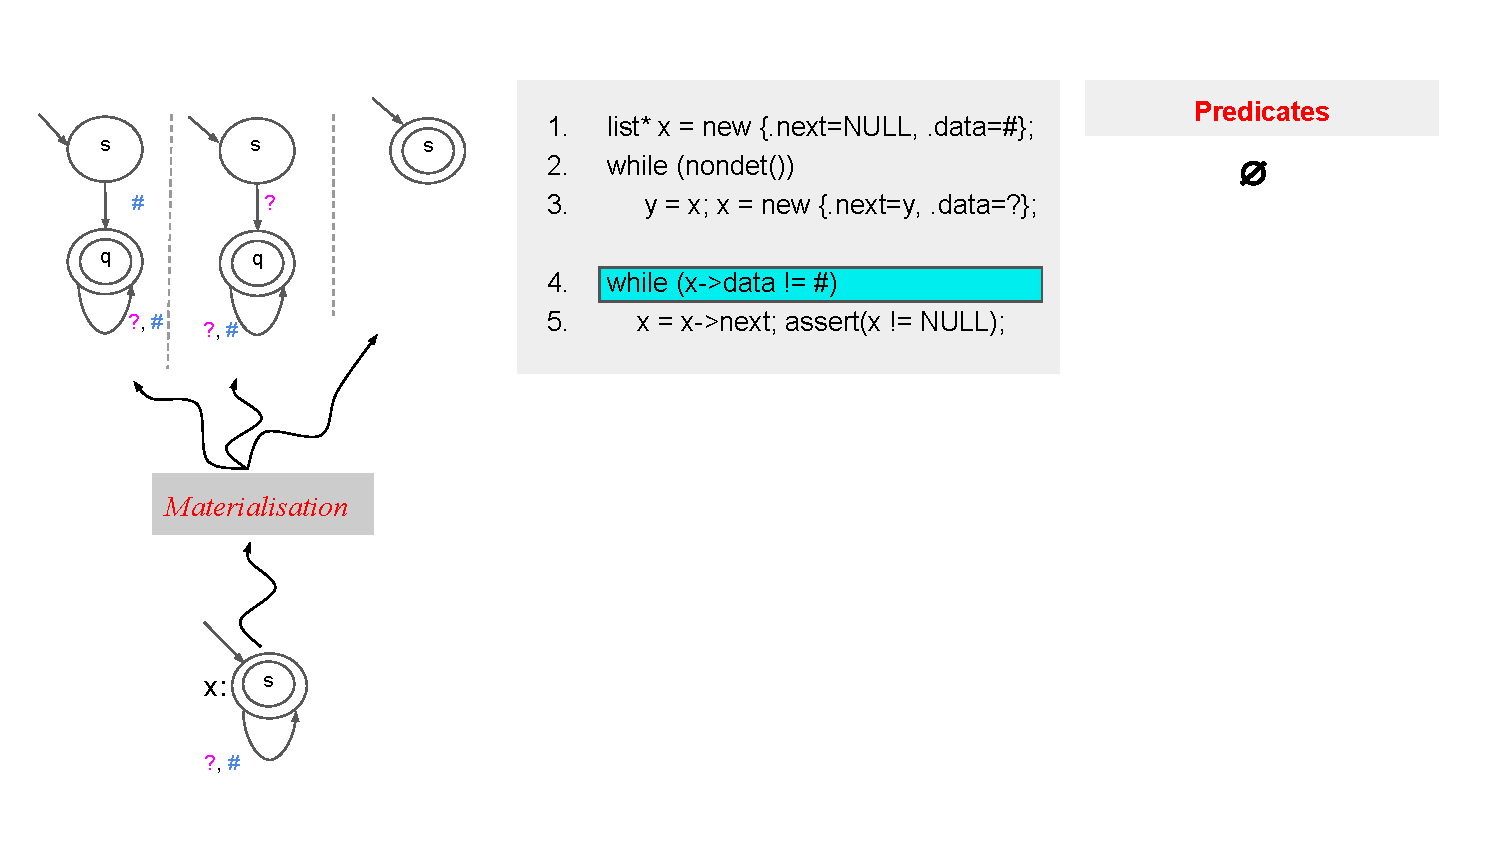
\includegraphics[scale=0.5]{ex/vmcai_8.pdf}}
      \only<9>{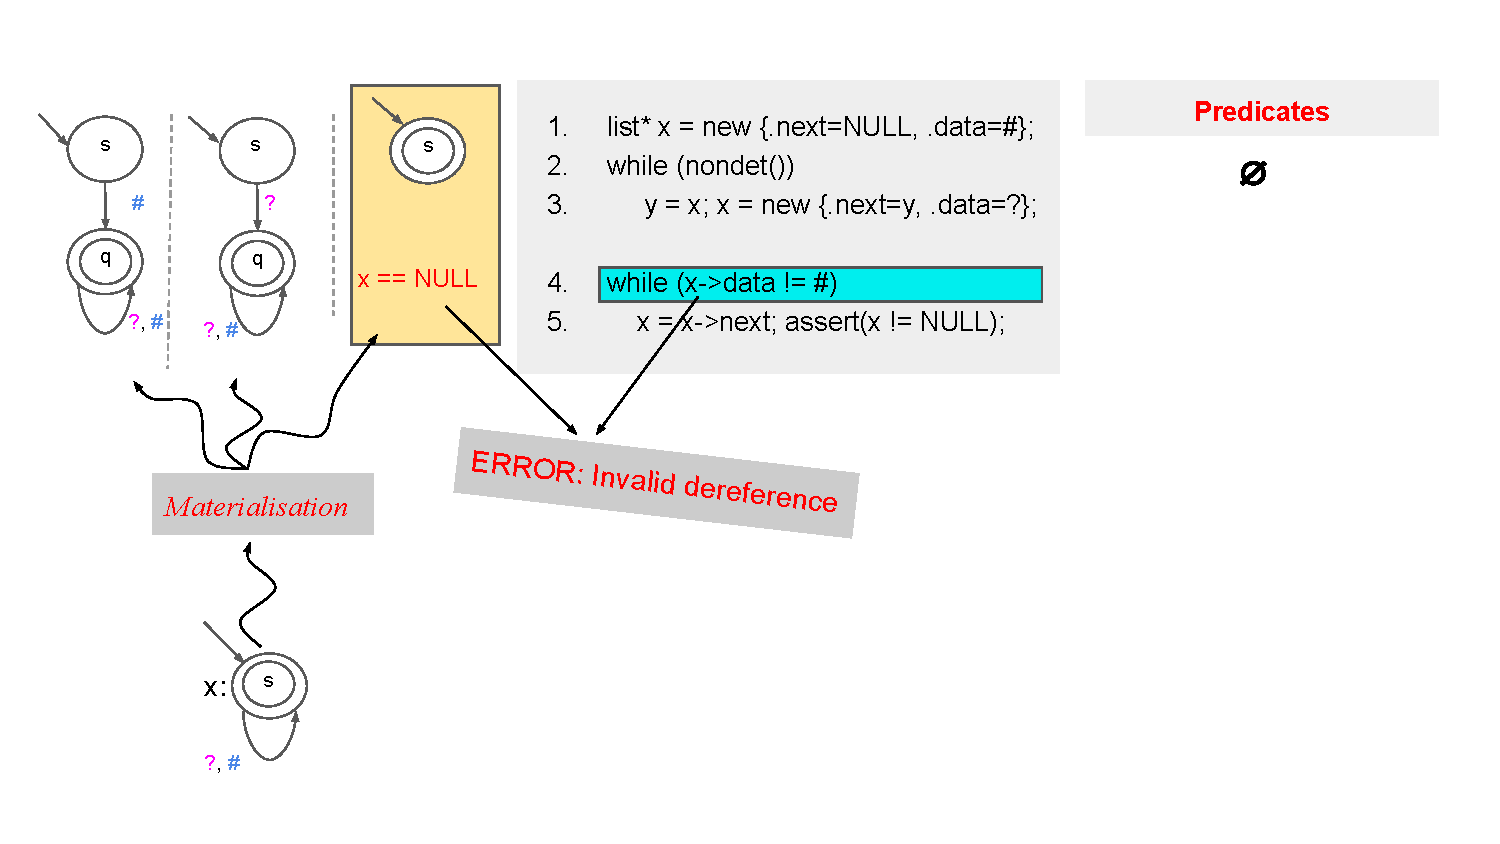
\includegraphics[scale=0.5]{ex/vmcai_9.pdf}}
    \end{overlayarea}
\end{frame}

%*******************************************************************************

%*******************************************************************************
\begin{frame}
% \begin{frame}[label=current]
  \frametitle{Example\,---\,Backward Run}
  \begin{overlayarea}{7cm}{6.5cm}
      \only<1>{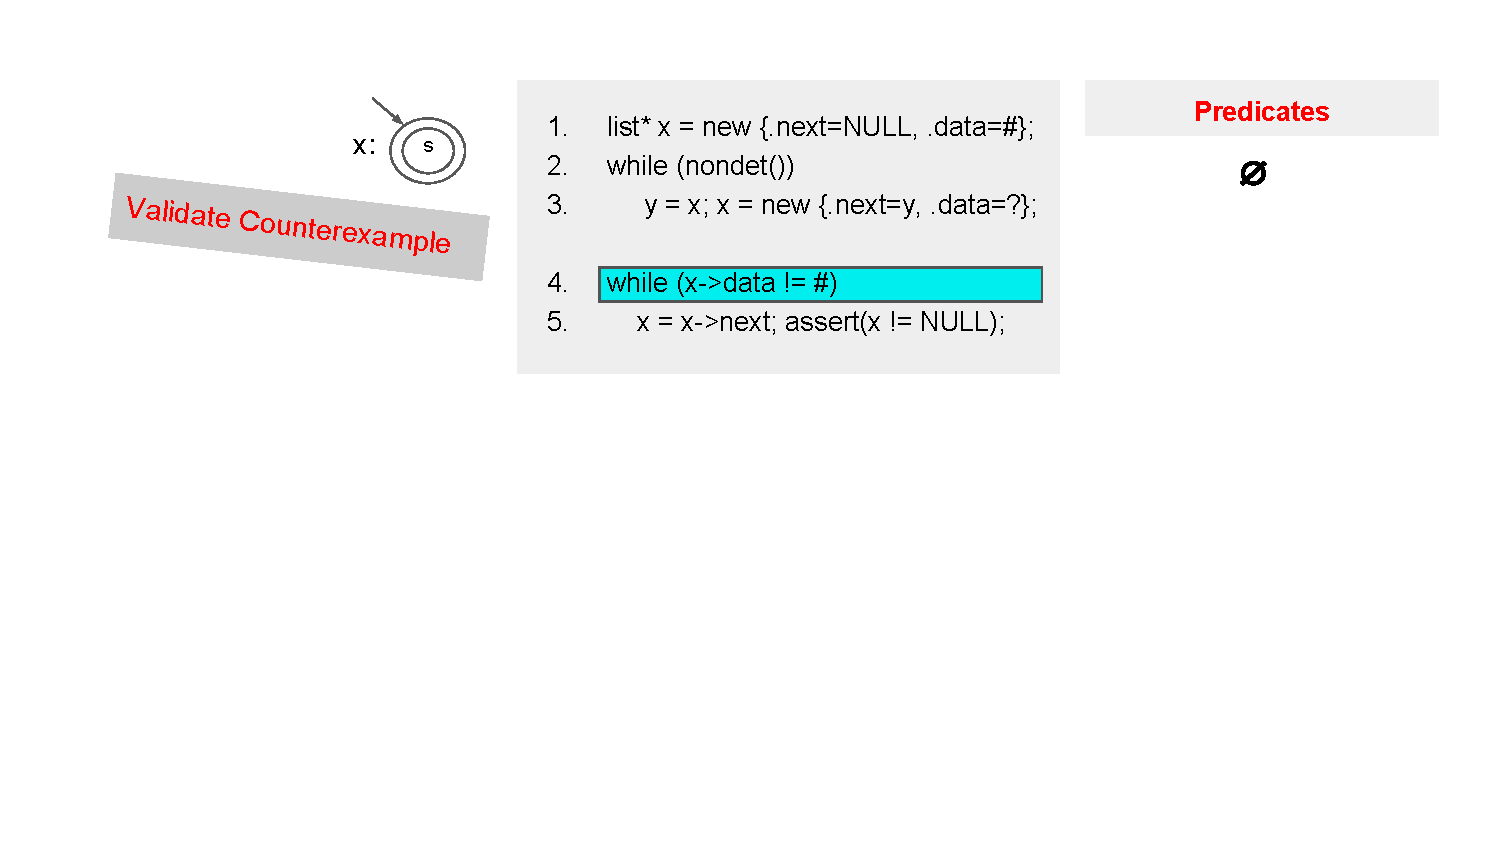
\includegraphics[scale=0.5]{ex/vmcai_10.pdf}}
      \only<2>{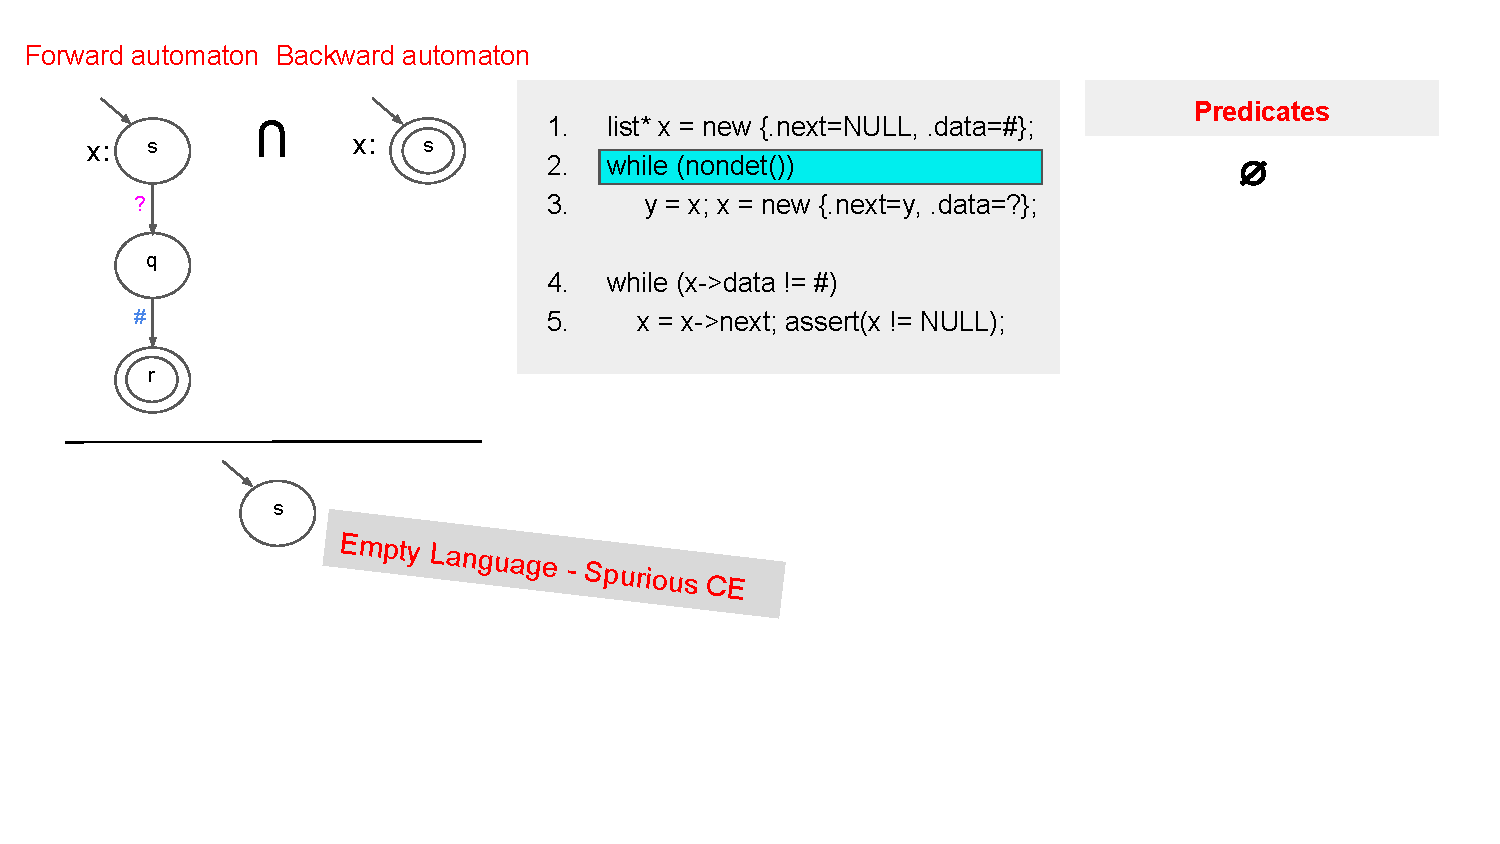
\includegraphics[scale=0.5]{ex/vmcai_11.pdf}}
      \only<3>{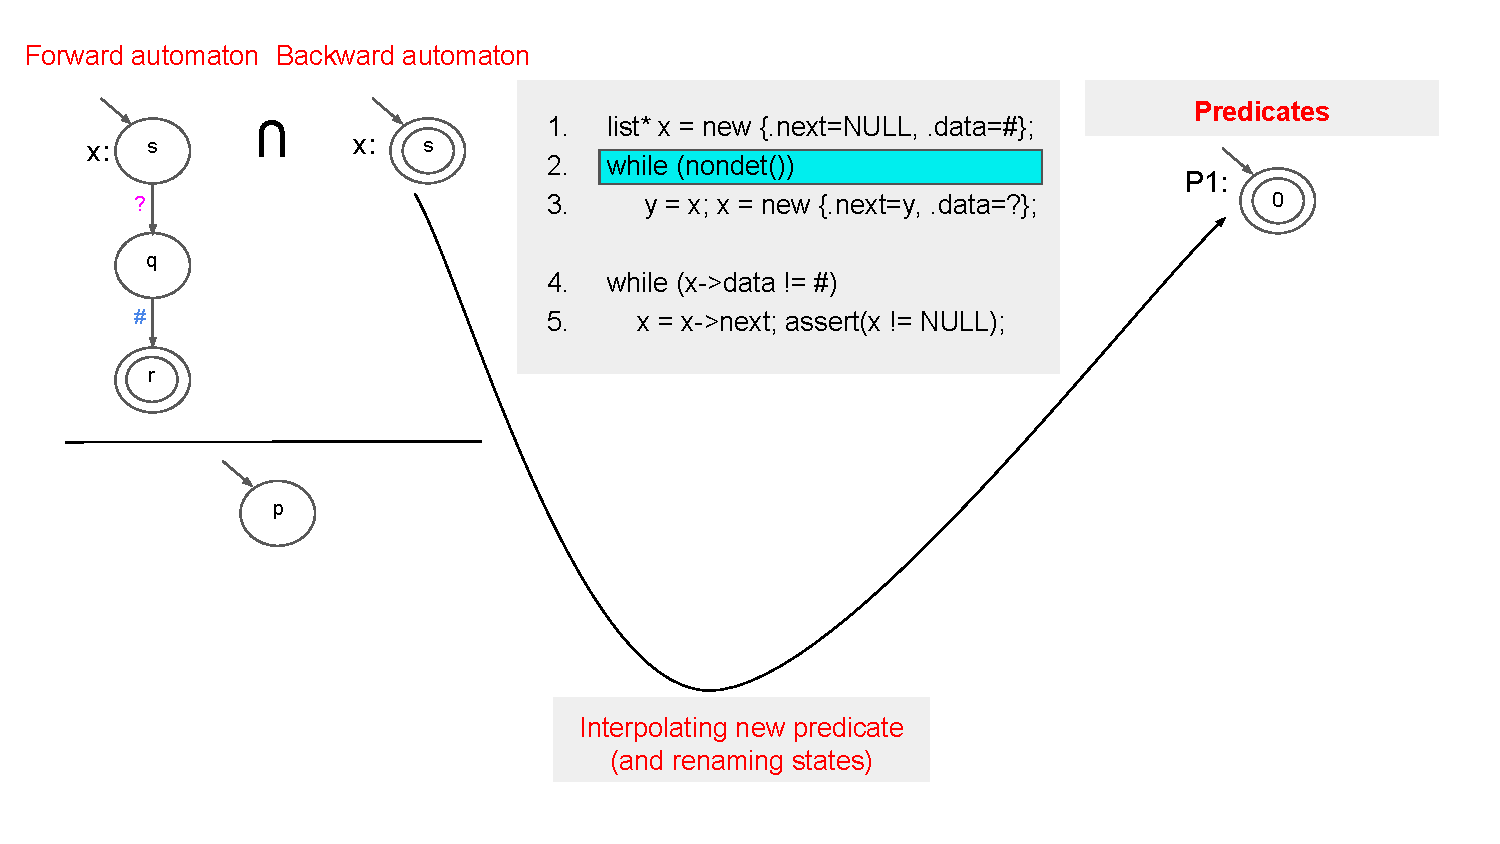
\includegraphics[scale=0.5]{ex/vmcai_12.pdf}}
  \end{overlayarea}
\end{frame}

%*******************************************************************************

%*******************************************************************************
\begin{frame}
% \begin{frame}[label=current]
  \frametitle{Example\,---\,Forward Run no. 2}
  \begin{overlayarea}{7cm}{6.5cm}
      \only<1>{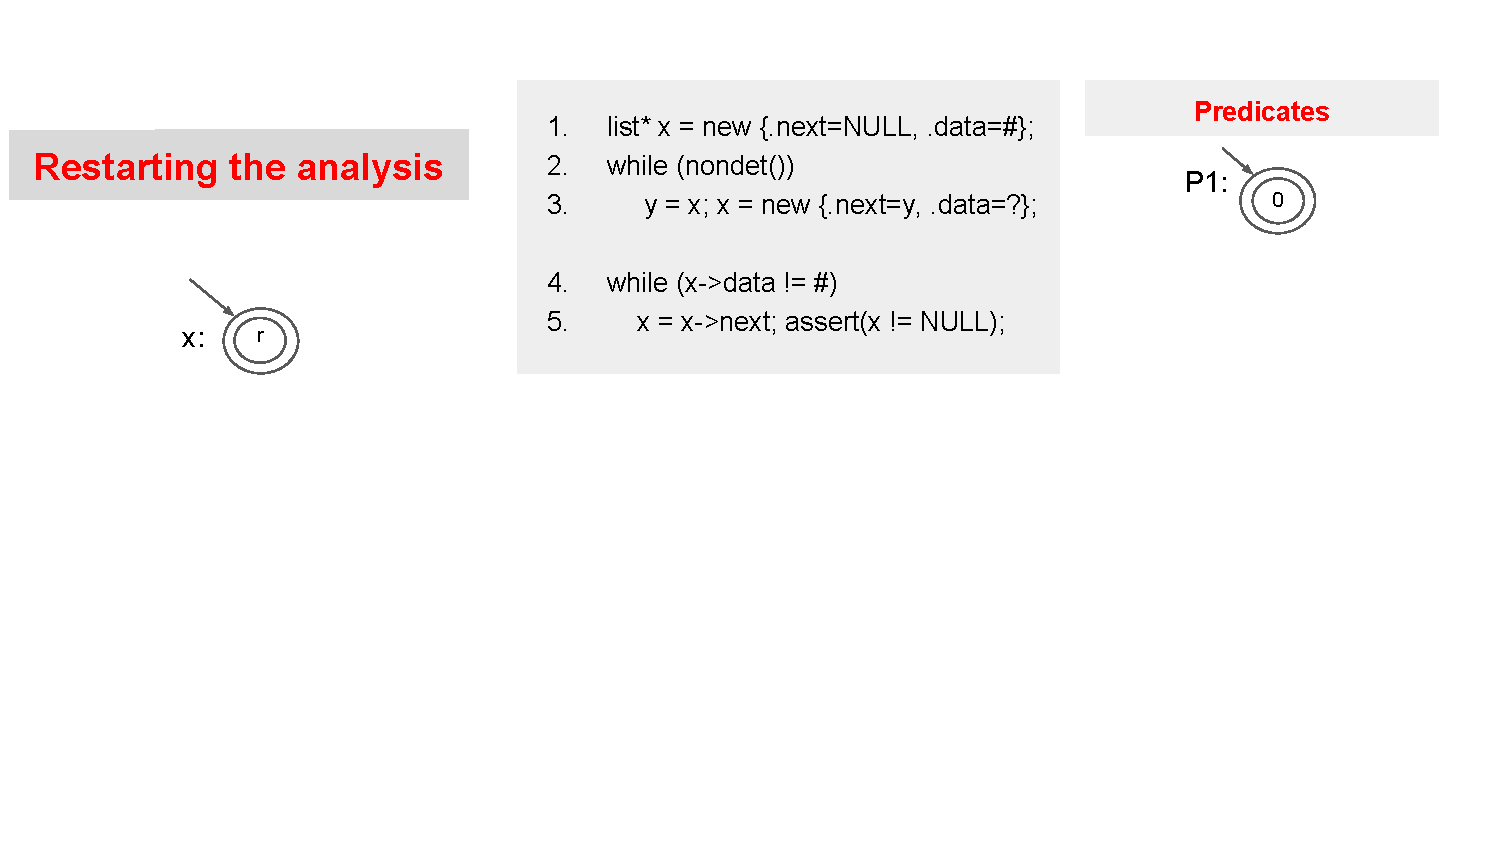
\includegraphics[scale=0.5]{ex/vmcai_13.pdf}}
      \only<2>{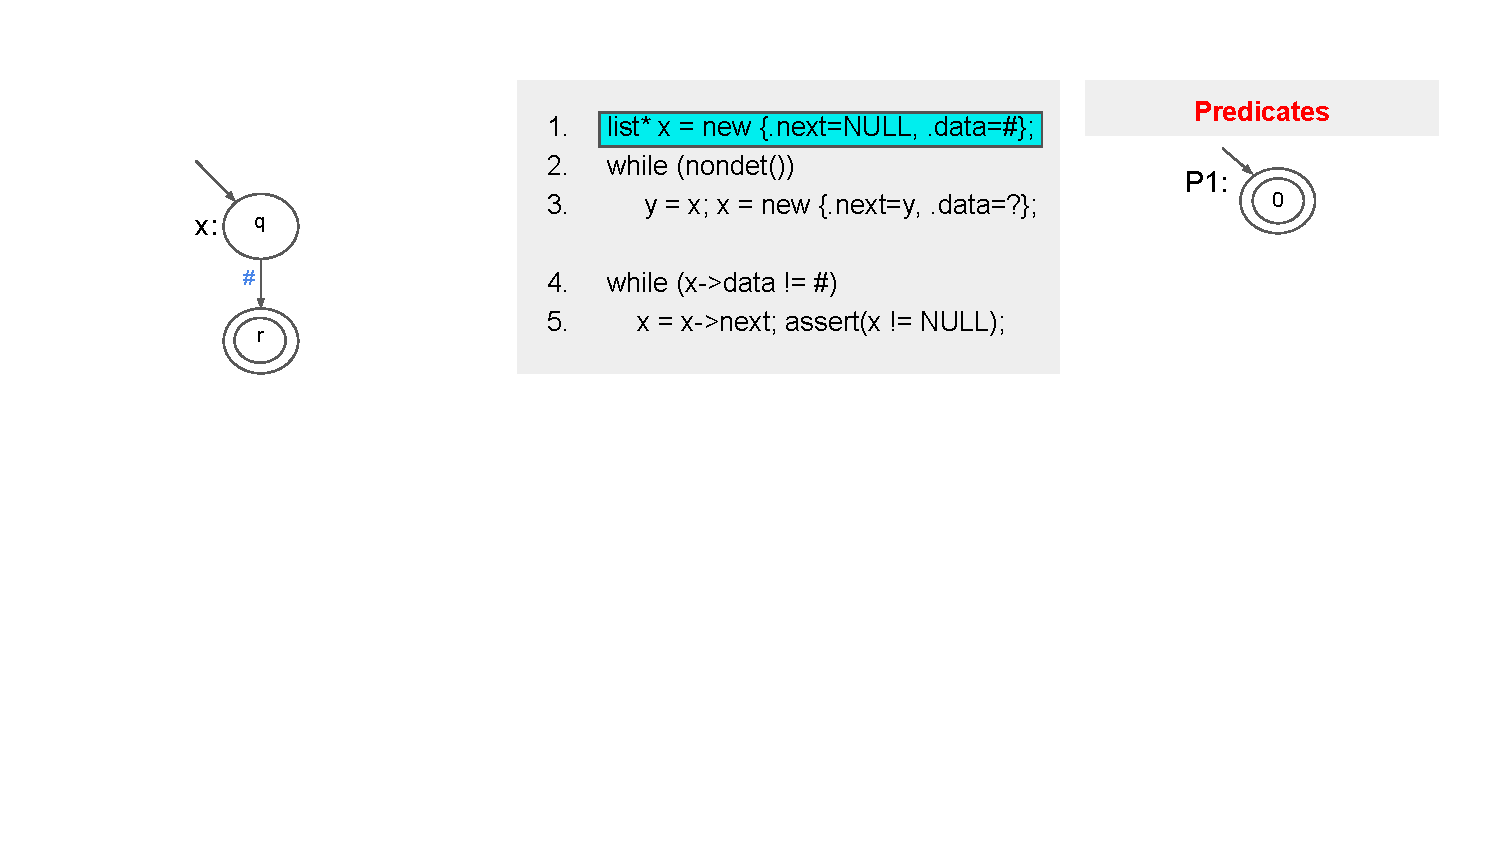
\includegraphics[scale=0.5]{ex/vmcai_14.pdf}}
      \only<3>{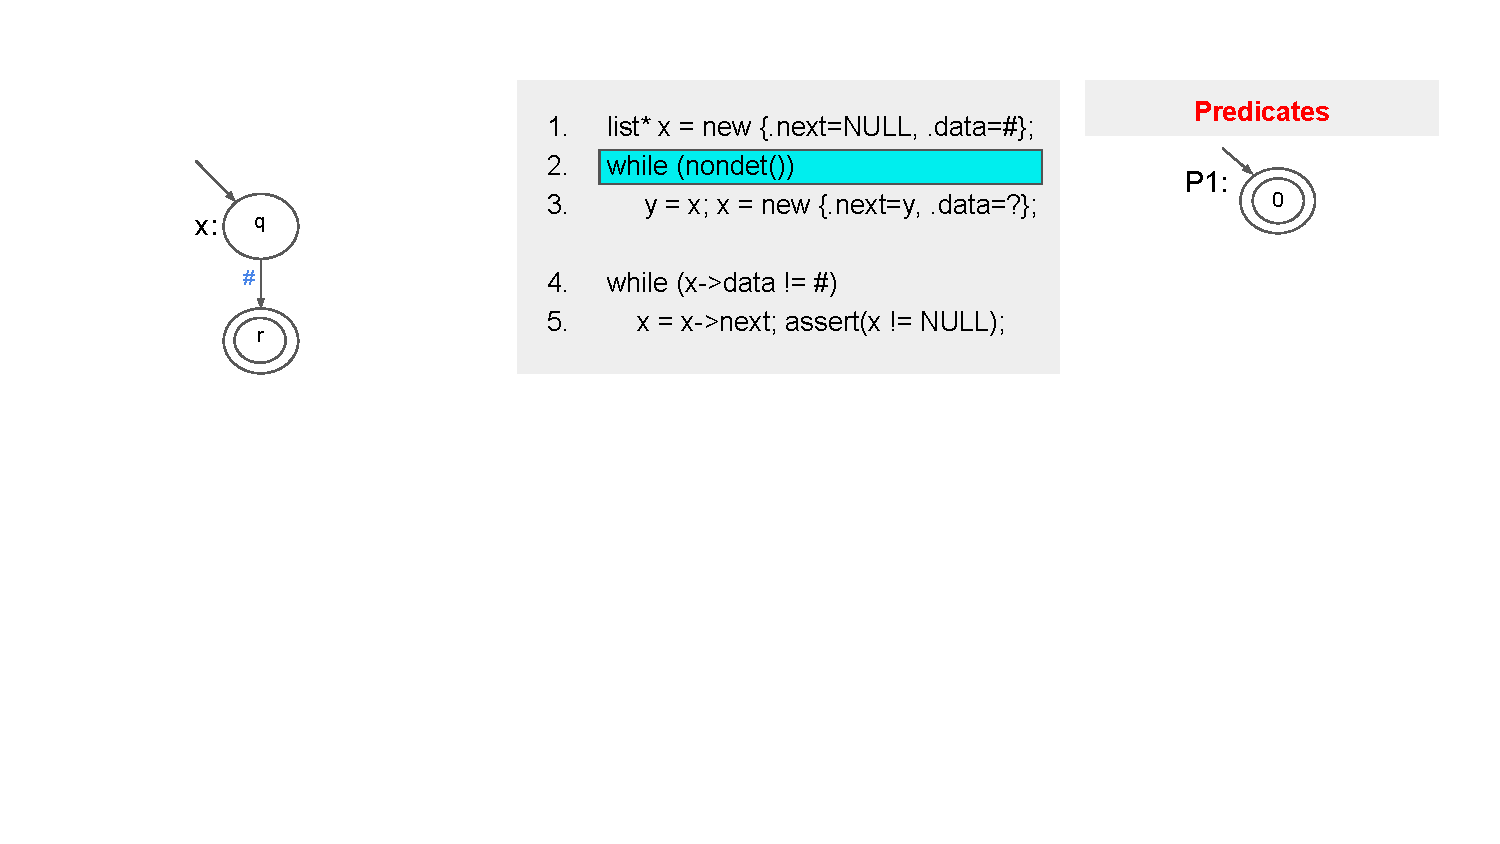
\includegraphics[scale=0.5]{ex/vmcai_15.pdf}}
      \only<4>{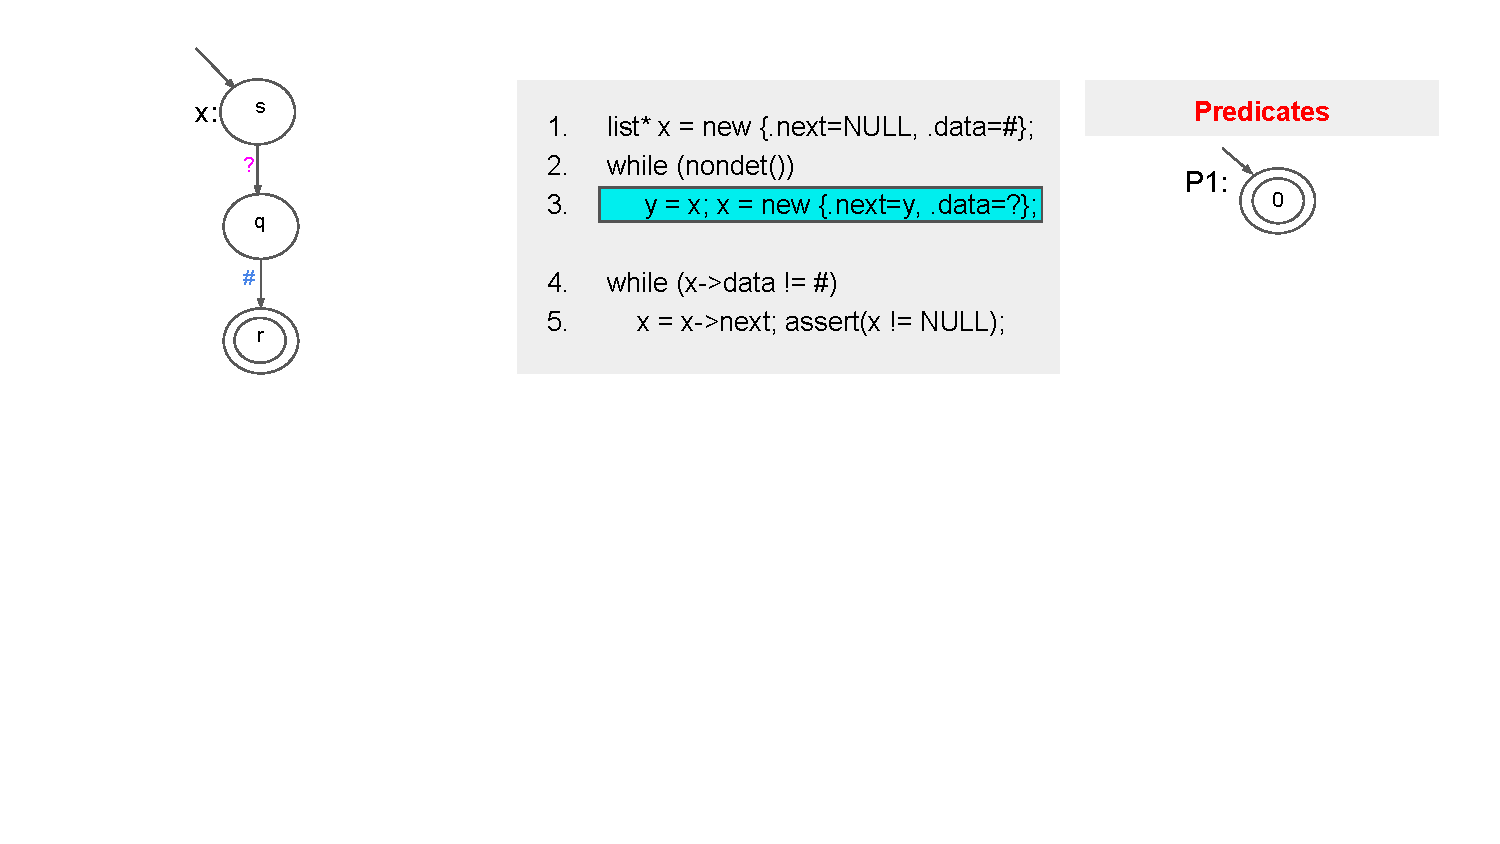
\includegraphics[scale=0.5]{ex/vmcai_16.pdf}}
      \only<5>{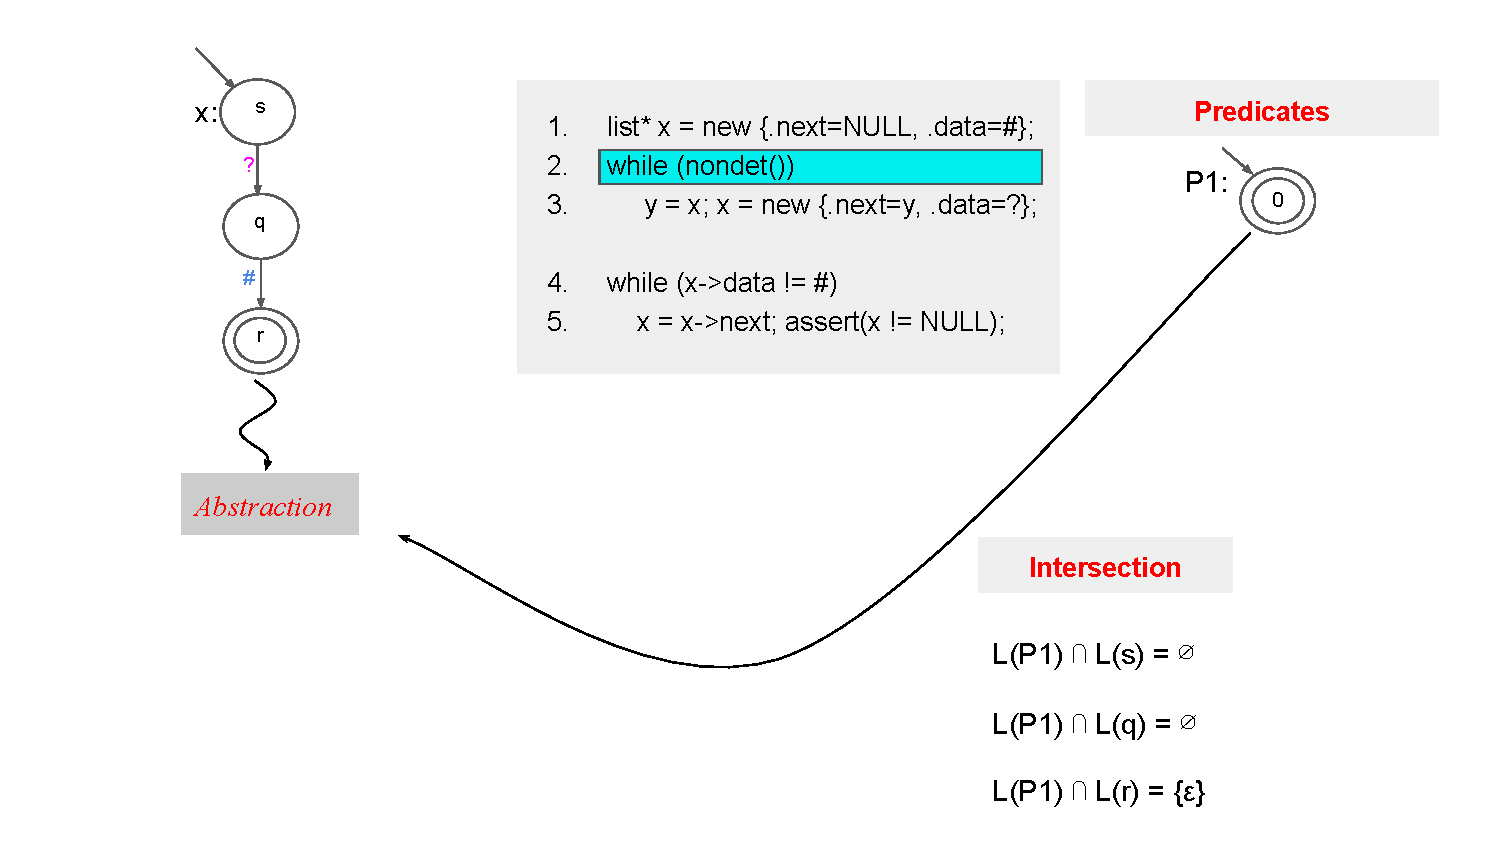
\includegraphics[scale=0.5]{ex/vmcai_17.pdf}}
      \only<6>{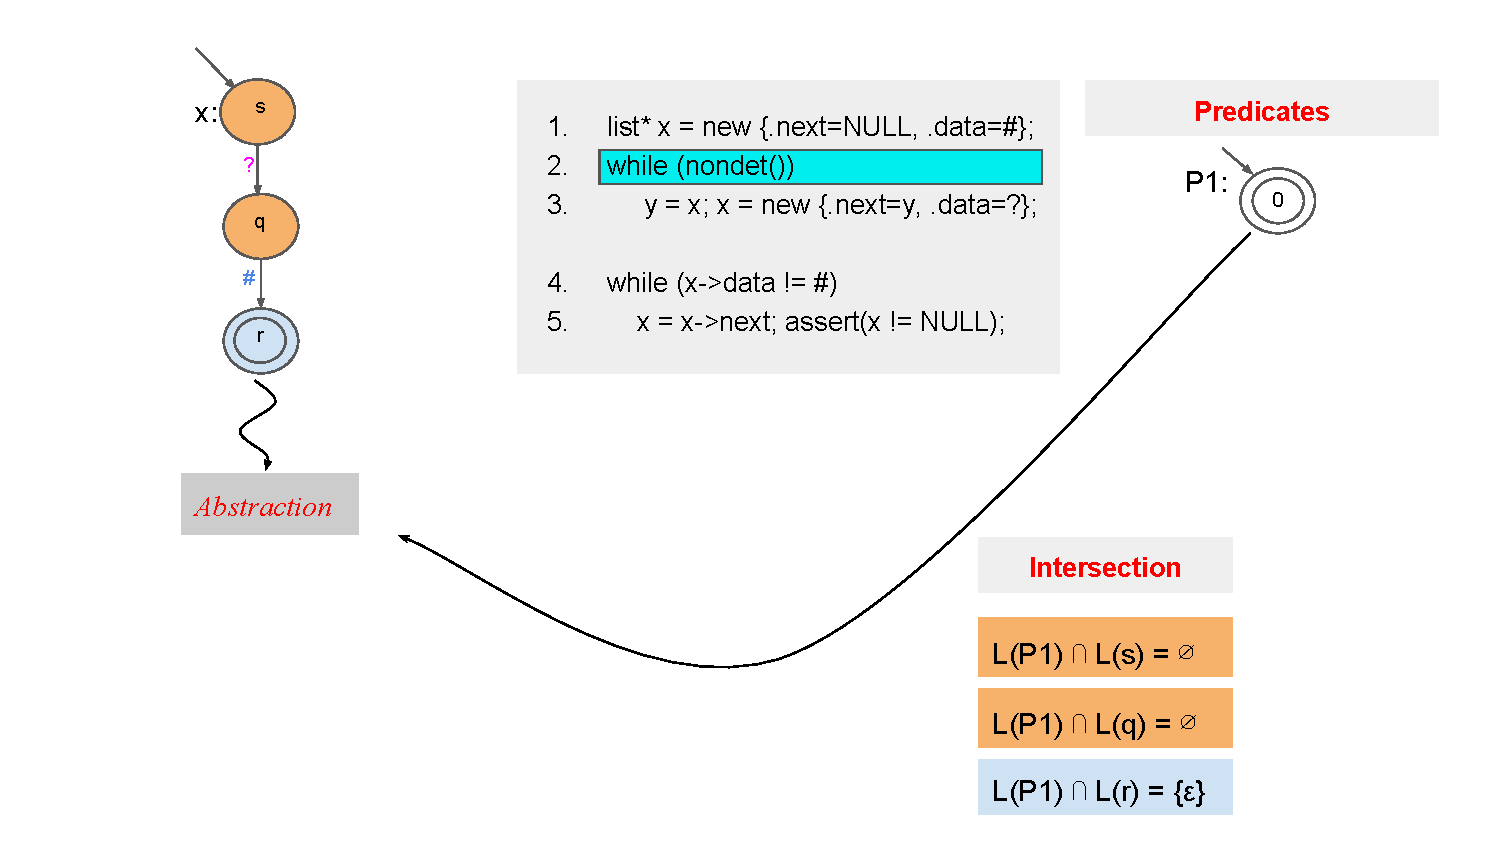
\includegraphics[scale=0.5]{ex/vmcai_18.pdf}}
      \only<7>{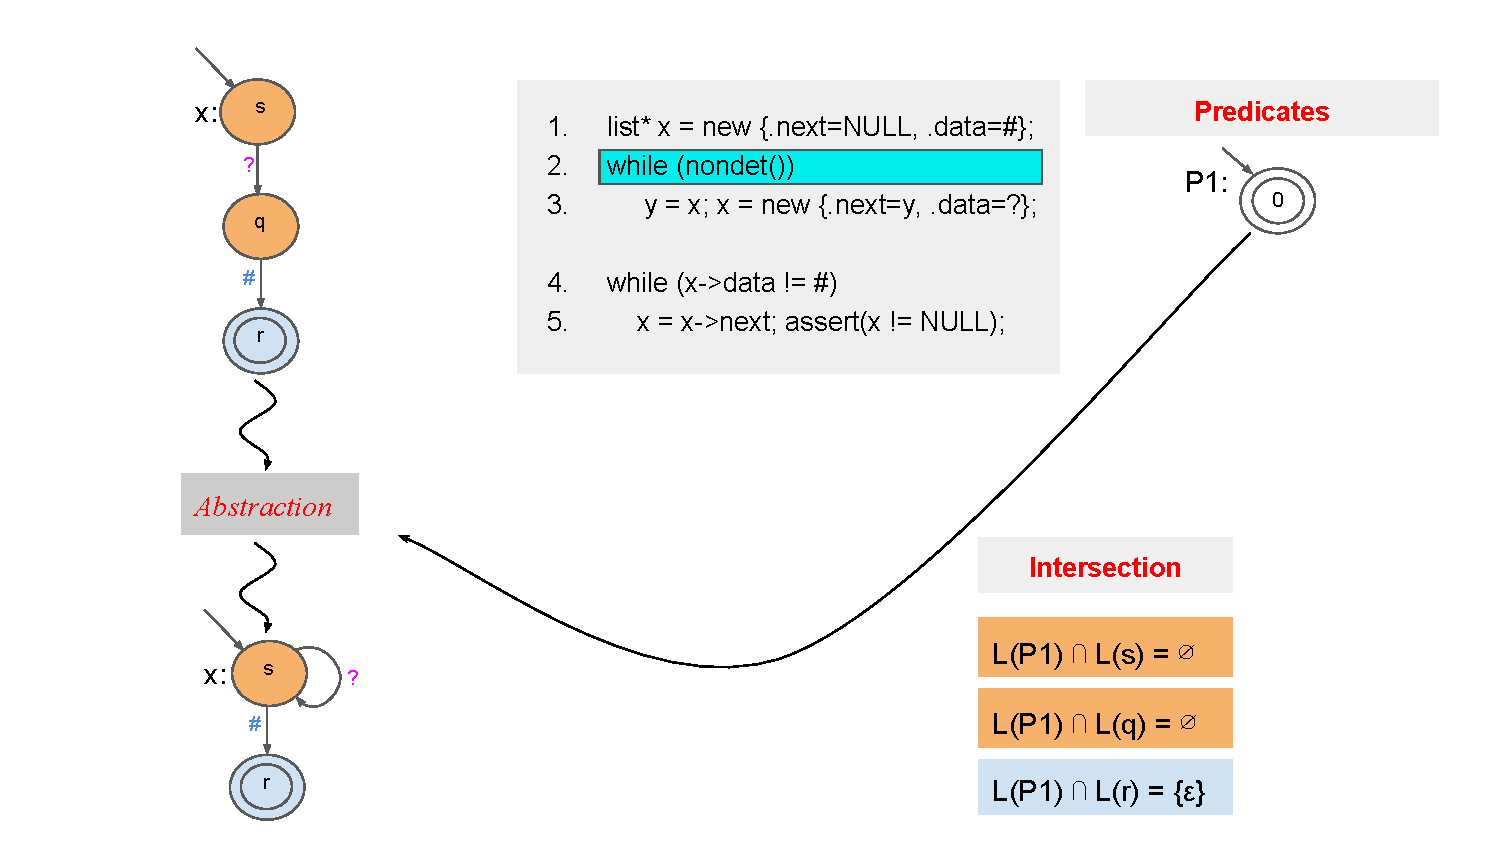
\includegraphics[scale=0.5]{ex/vmcai_19.pdf}}
	  \only<8>{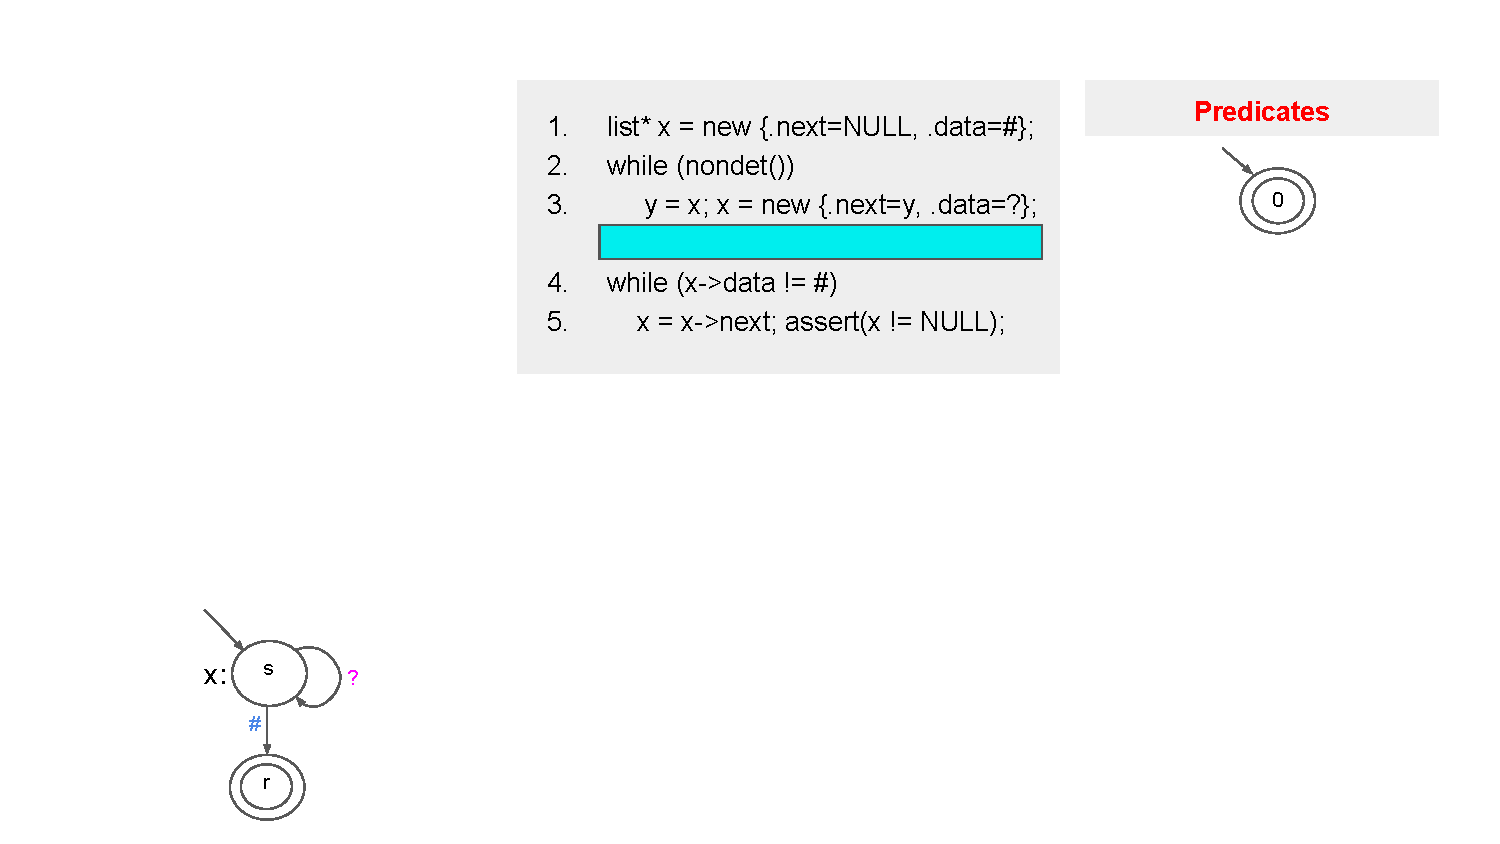
\includegraphics[scale=0.5]{ex/vmcai_20.pdf}}
	  \only<9>{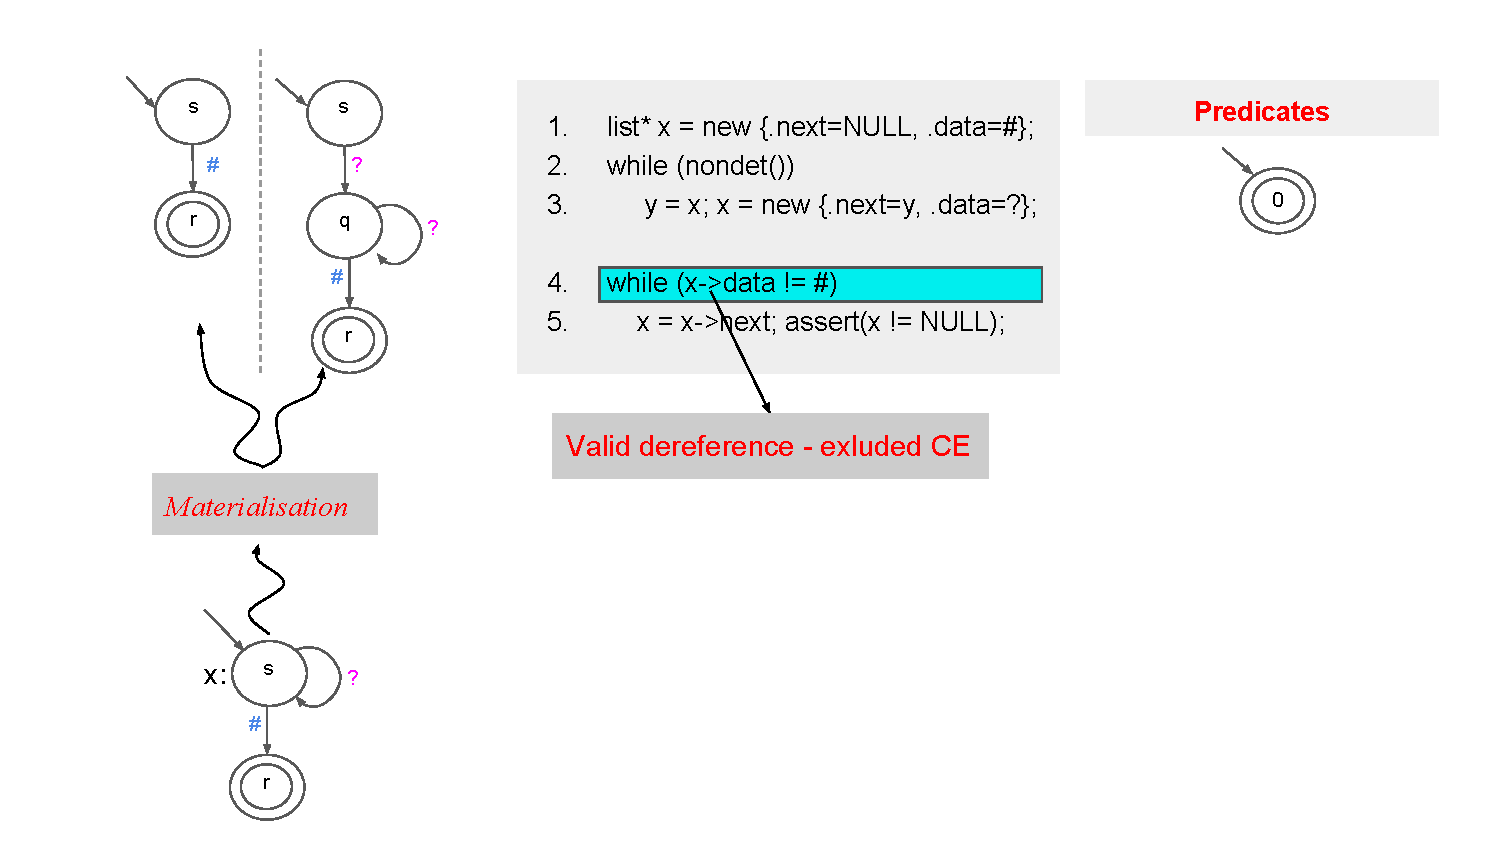
\includegraphics[scale=0.5]{ex/vmcai_21.pdf}}
      \only<10>{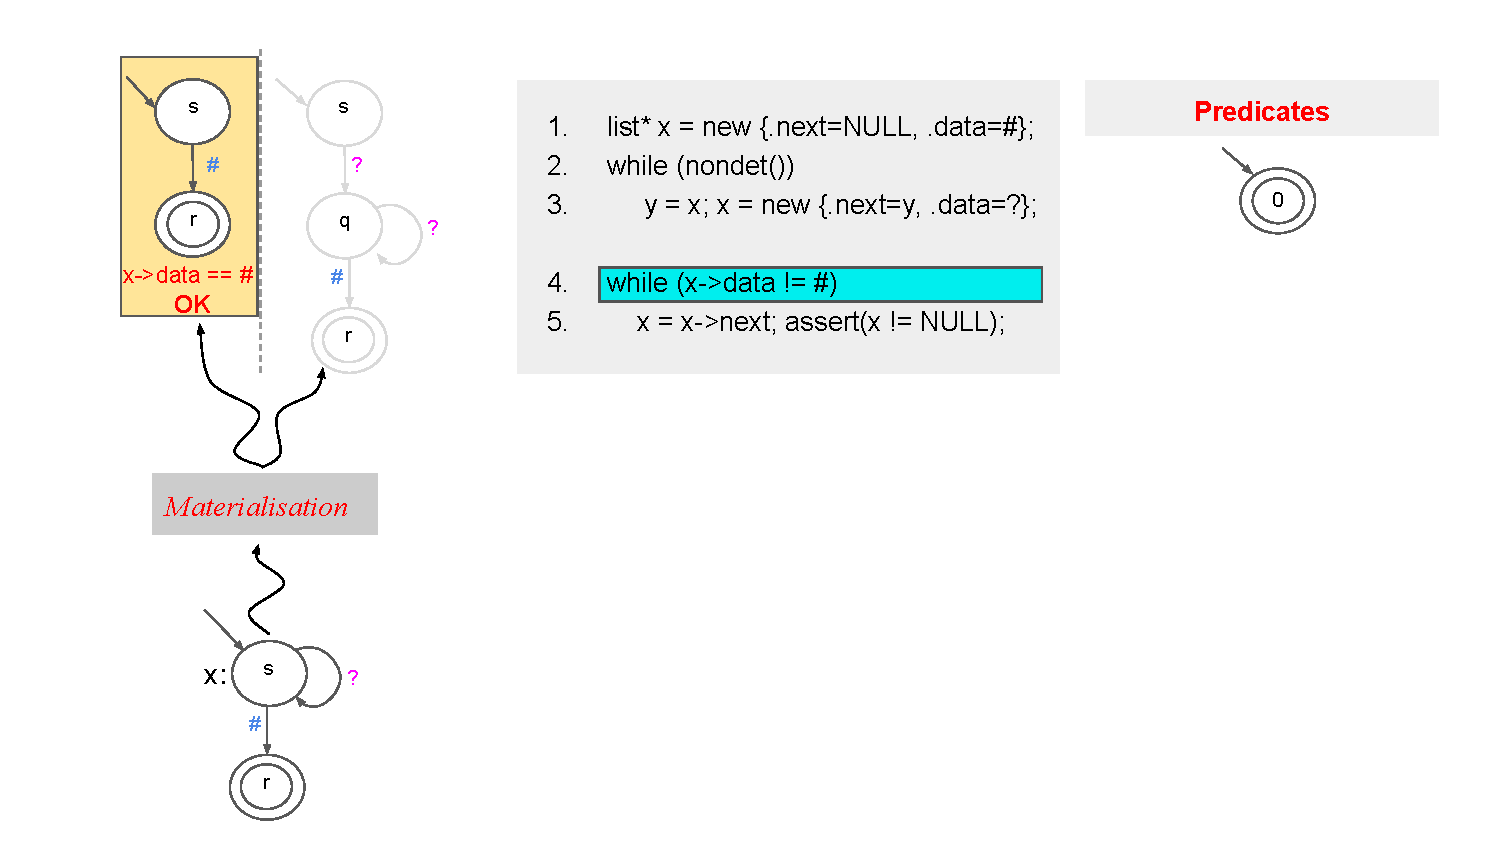
\includegraphics[scale=0.5]{ex/vmcai_22.pdf}}
      \only<11>{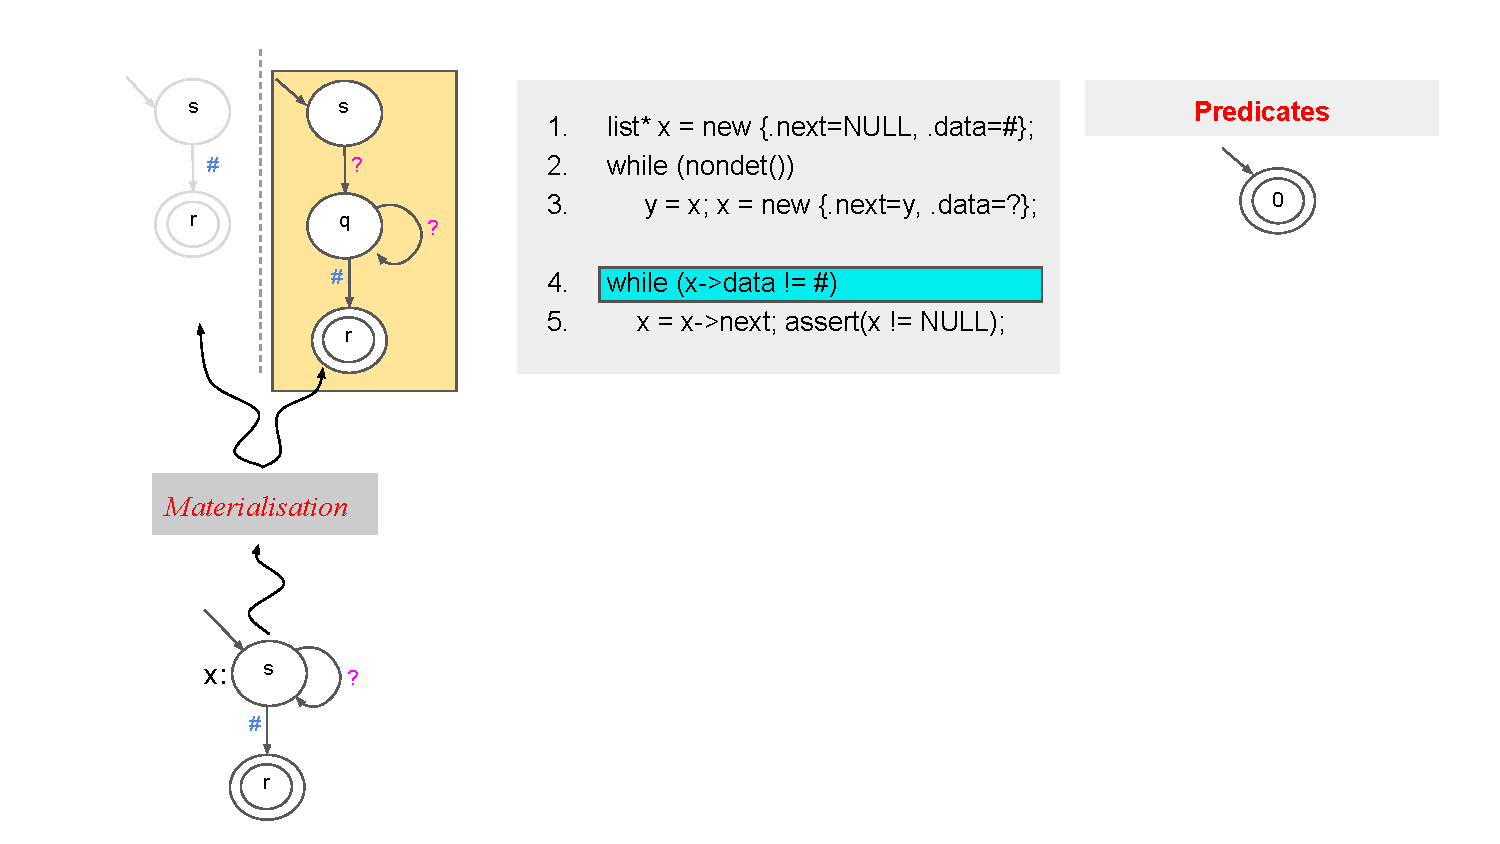
\includegraphics[scale=0.5]{ex/vmcai_23.pdf}}
      \only<12>{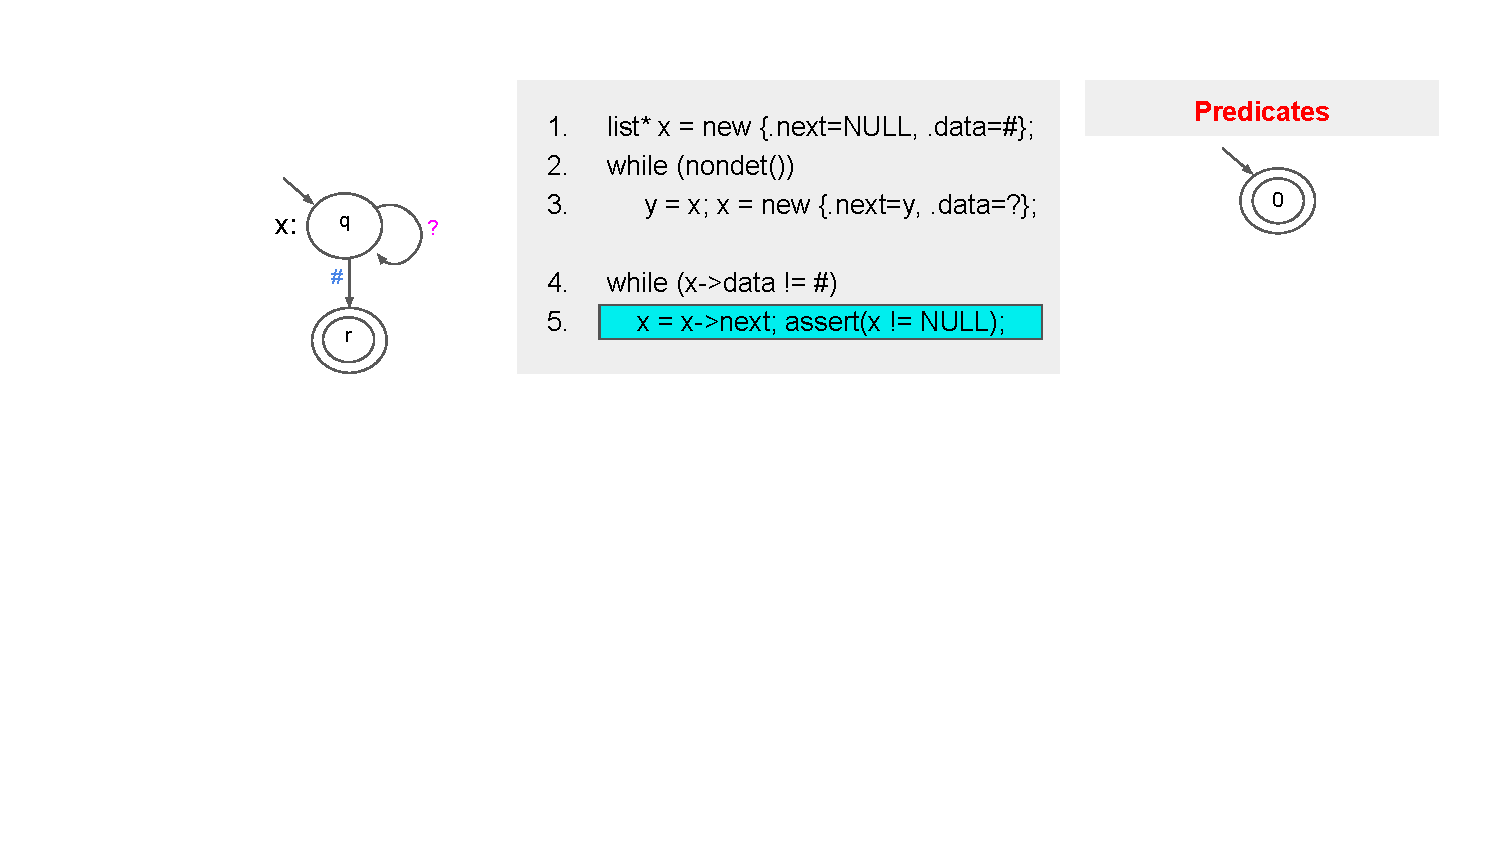
\includegraphics[scale=0.5]{ex/vmcai_24.pdf}}
      \only<13>{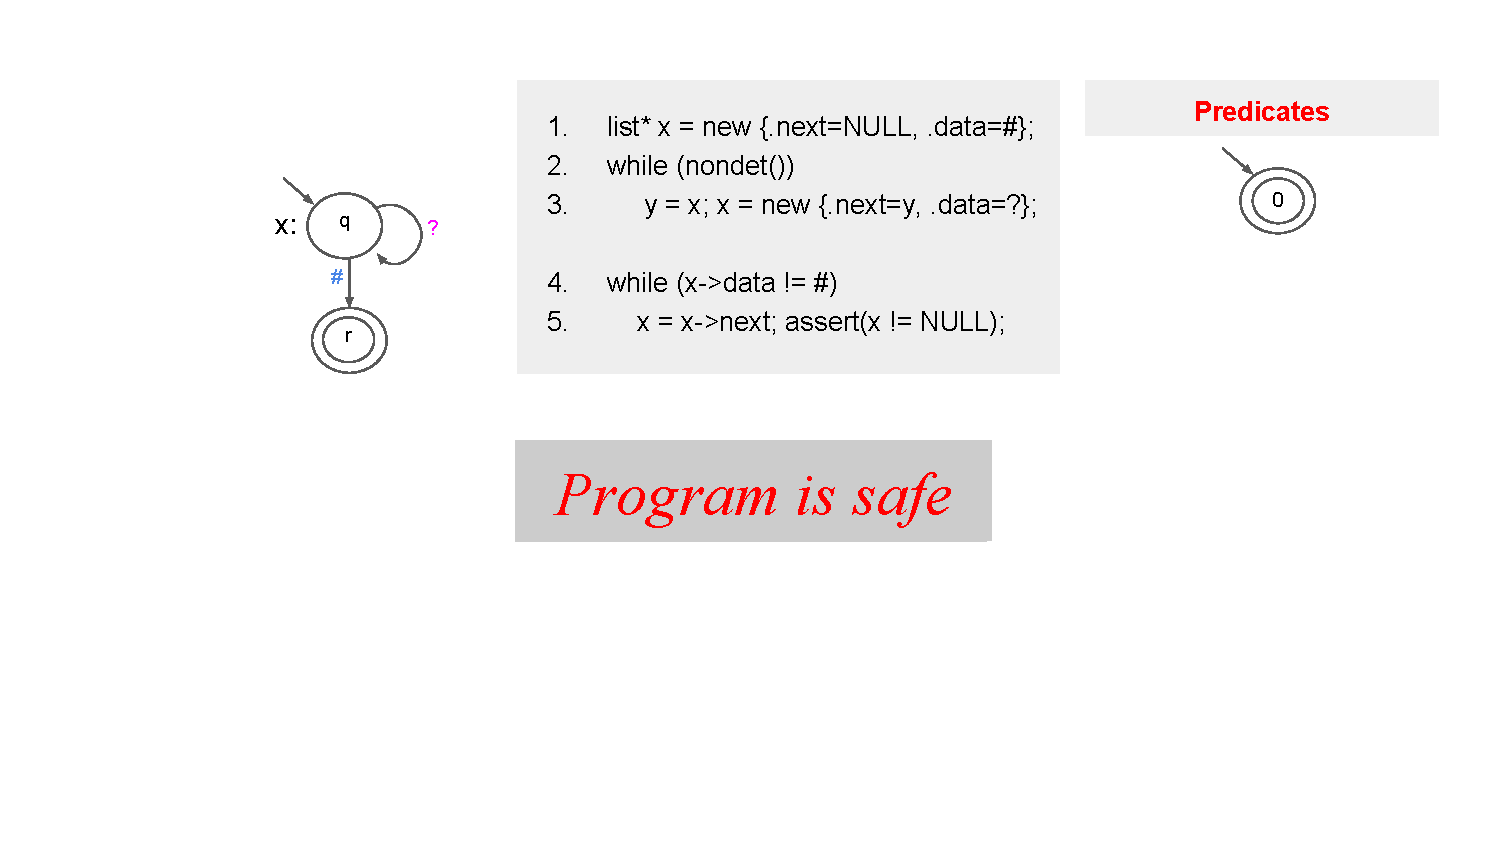
\includegraphics[scale=0.5]{ex/vmcai_25.pdf}}
    \end{overlayarea}
\end{frame}

%*******************************************************************************
%*******************************************************************************
\begin{frame}
\frametitle{Forest Automata Encoding of Heap}

	\begin{itemize}
			\item An \hlbl{FA} is a tuple of \hlgr{tree automata (TA)}
				\pause
			\item A \hlgr{TA} accepts \hlrd{trees}
				\pause
			\item \hlrd{Trees} can contain leaves referencing the roots of other trees
				\pause
			\item An FA $F=(TA_1,\ldots,TA_n)$ represent \hlrd{tree decompositions} (tuples of trees $t_1,\ldots,t_n$) of heap graphs
				such that $\forall 1 \leq i \leq n: t_i \in L(TA_i)$
				\pause
			\item Encoded heap graphs obtained by connecting leaves with the~referenced roots
			%\item \hlye{Cut-points} are nodes of heap referenced by a variable or nodes with more than one incoming edges.
	\end{itemize}

	\begin{center}
	\tikzset{every picture/.style={scale=0.8}}%
	\begin{figure*}
		\begin{subfigure}{0.5\textwidth}
			\centering
			\usetikzlibrary{calc,matrix,backgrounds,fit,shapes,arrows,patterns}
\begin{tikzpicture}[
  scale=0.8,
  transform shape,
  node distance=18mm
]

  \tikzstyle{memnode}=[draw,rectangle,fill=lightgray,thick,minimum height=4.5mm, minimum width=4.5mm,inner sep=1mm,node distance=18mm,font=\tt]
  \tikzstyle{memnodeblue}=[draw,rectangle,fill=blue!30,thick,minimum height=4.5mm, minimum width=4.5mm,inner sep=1mm,node distance=18mm,font=\tt]
  \tikzstyle{memnodepink}=[draw,rectangle,fill=red!30,thick,minimum height=4.5mm, minimum width=4.5mm,inner sep=1mm,node distance=18mm,font=\tt]
  \tikzstyle{memnodegreen}=[draw,rectangle,fill=green!60,thick,minimum height=4.5mm, minimum width=4.5mm,inner sep=1mm,node distance=18mm,font=\tt]

  \tikzstyle{nullnode}=[node distance=18mm,label=center:$\bot$]
  \tikzstyle{varnode}=[font=\tt]
  \tikzstyle{refnode}=[fill=green!20,minimum height=4.5mm, minimum width=4.5mm,inner sep=1mm,font=\tt]

  \tikzstyle{pointer}=[draw,->,>=latex]
  \tikzstyle{ptrlab}=[above,font=\tt]
  \tikzstyle{rightptr}=[label={[label distance=-1mm,font=\tt,rotate=37]90:right}]
  \tikzstyle{rightptr0}=[label={[label distance=-1mm,font=\tt,rotate=31]90:right}]
  \tikzstyle{leftptr}=[label={[label distance=-1mm,font=\tt,rotate=-37]90:left}]
  \tikzstyle{leftptr1}=[label={[label distance=-1mm,font=\tt,rotate=-45]90:left}]
  \tikzstyle{leftptr0}=[label={[label distance=-1mm,font=\tt,rotate=-31]90:left}]

  % nodes
  \node[memnodeblue] (x1) at (0mm,0mm) {1};
  \node[memnodeblue] (x2) [right of=x1] {};
  \node[memnodeblue] (x3) [above right of=x2,yshift=-3mm] {};
  \node[nullnode] (x3null1) [above right of=x3,yshift=-5mm] {};
  \node[nullnode] (x3null2) [below right of=x3,yshift=5mm] {};

  \node[memnodepink] (y1) [below of=x1] {3};
  \node[memnodepink] (y2) [right of=y1] {};

  \node[refnode] (joinsbst1) [below right of=x2,yshift=3mm] {\=2};
  \node[refnode] (joinsbst2) [right of=y2] {\=2};


  \node[memnodegreen] (join) [right of=joinsbst2,xshift=-6mm] {2};
  \node[memnodegreen] (j2) [above right of=join,yshift=-3mm] {};
  \node[memnodegreen] (j3) [below right of=join,yshift=3mm] {};
  \node[nullnode] (j2null1) [above right of=j2,yshift=-5mm] {};
  \node[nullnode] (j2null2) [below right of=j2,yshift=5mm] {};
  \node[nullnode] (j3null1) [above right of=j3,yshift=-5mm] {};
  \node[nullnode] (j3null2) [below right of=j3,yshift=5mm] {};

  \node[varnode,node distance=5mm] (x) [left of=x1] {x:};
  \node[varnode,node distance=5mm] (x) [left of=y1] {y:};

  % pointers
  \draw[pointer] (x1)    -- node[ptrlab]   {next} (x2);
  \draw[pointer] (x2)    -- node[rightptr] {}     (x3);
  \draw[pointer] (x3)    -- node[rightptr0]{}     (x3null1);
  \draw[pointer] (x3)    -- node[leftptr0] {}     (x3null2);
  \draw[pointer] (x2)    -- node[leftptr] {}     (joinsbst1);

  \draw[pointer] (y1)    -- node[ptrlab]   {next} (y2);
  \draw[pointer] (y2)    -- node[ptrlab]   {next} (joinsbst2);

  \draw[pointer] (join) -- node[rightptr]  {}     (j2);
  \draw[pointer] (j2)   -- node[rightptr0] {}     (j2null1);
  \draw[pointer] (j2)   -- node[leftptr0]  {}     (j2null2);
  \draw[pointer] (join) -- node[leftptr]   {}     (j3);
  \draw[pointer] (j3)   -- node[rightptr0] {}     (j3null1);
  \draw[pointer] (j3)   -- node[leftptr0]  {}     (j3null2);

\end{tikzpicture}

		\end{subfigure}%
		\hspace{-0.3cm}
		\begin{subfigure}{0.5\textwidth}
			\centering
			\usetikzlibrary{calc,matrix,backgrounds,fit,shapes,arrows}
\begin{tikzpicture}[
  scale=0.8,
  transform shape,
]

  \tikzstyle{memnode}=[draw,rectangle,fill=lightgray,thick,minimum height=4.5mm, minimum width=4.5mm,inner sep=1mm,node distance=18mm,font=\tt]
  \tikzstyle{memnodeblue}=[draw,rectangle,fill=blue!30,thick,minimum height=4.5mm, minimum width=4.5mm,inner sep=1mm,node distance=18mm,font=\tt]
  \tikzstyle{memnodepink}=[draw,rectangle,fill=red!30,thick,minimum height=4.5mm, minimum width=4.5mm,inner sep=1mm,node distance=18mm,font=\tt]
  \tikzstyle{memnodegreen}=[draw,rectangle,fill=green!60,thick,minimum height=4.5mm, minimum width=4.5mm,inner sep=1mm,node distance=18mm,font=\tt]

  \tikzstyle{nullnode}=[node distance=18mm,label=center:$\bot$]
  \tikzstyle{varnode}=[font=\tt]

  \tikzstyle{pointer}=[draw,->,>=latex]
  \tikzstyle{ptrlab}=[above,font=\tt]
  \tikzstyle{rightptr}=[label={[label distance=-1mm,font=\tt,rotate=37]90:right}]
  \tikzstyle{rightptr0}=[label={[label distance=-1mm,font=\tt,rotate=31]90:right}]
  \tikzstyle{leftptr}=[label={[label distance=-1mm,font=\tt,rotate=-37]90:left}]
  \tikzstyle{leftptr1}=[label={[label distance=-1mm,font=\tt,rotate=-45]90:left}]
  \tikzstyle{leftptr0}=[label={[label distance=-1mm,font=\tt,rotate=-31]90:left}]

  % nodes
  \node[memnodeblue] (x1) at (0mm,0mm) {1};
  \node[memnodeblue] (x2) [right of=x1] {};
  \node[memnodeblue] (x3) [above right of=x2,yshift=-3mm] {};
  \node[nullnode] (x3null1) [above right of=x3,yshift=-5mm] {};
  \node[nullnode] (x3null2) [below right of=x3,yshift=5mm] {};

  \node[memnodepink] (y1) [below of=x1] {3};
  \node[memnodepink] (y2) [right of=y1] {};

  \node[memnodegreen] (join) [right of=y2] {2};
  \node[memnodegreen] (j2) [above right of=join,yshift=-3mm] {};
  \node[memnodegreen] (j3) [below right of=join,yshift=3mm] {};
  \node[nullnode] (j2null1) [above right of=j2,yshift=-5mm] {};
  \node[nullnode] (j2null2) [below right of=j2,yshift=5mm] {};
  \node[nullnode] (j3null1) [above right of=j3,yshift=-5mm] {};
  \node[nullnode] (j3null2) [below right of=j3,yshift=5mm] {};

  \node[varnode,node distance=5mm] (x) [left of=x1] {x:};
  \node[varnode,node distance=5mm] (x) [left of=y1] {y:};

  % pointers
  \draw[pointer] (x1)    -- node[ptrlab]   {next} (x2);
  \draw[pointer] (x2)    -- node[rightptr] {}     (x3);
  \draw[pointer] (x3)    -- node[rightptr0]{}     (x3null1);
  \draw[pointer] (x3)    -- node[leftptr0] {}     (x3null2);
  \draw[pointer] (x2)    -- node[leftptr1] {}     (join);

  \draw[pointer] (y1)    -- node[ptrlab]   {next} (y2);
  \draw[pointer] (y2)    -- node[ptrlab]   {next} (join);

  \draw[pointer] (join) -- node[rightptr]  {}     (j2);
  \draw[pointer] (j2)   -- node[rightptr0] {}     (j2null1);
  \draw[pointer] (j2)   -- node[leftptr0]  {}     (j2null2);
  \draw[pointer] (join) -- node[leftptr]   {}     (j3);
  \draw[pointer] (j3)   -- node[rightptr0] {}     (j3null1);
  \draw[pointer] (j3)   -- node[leftptr0]  {}     (j3null2);

\end{tikzpicture}

		\end{subfigure}
	\end{figure*}
	\end{center}

\end{frame}

%*******************************************************************************

%*******************************************************************************
\begin{frame}
\frametitle{Abstraction}

	\begin{itemize}
		\item Overapproximates reachable configurations and accelerates analysis
		\item Collapses states in the same equivalence class of \hlrd{a relation $\sim$}
		\item \hlgr{Height Abstraction}
		\begin{itemize}
			\item Consider states $q_1, q_2$, equivalence $\sim_H$ is defined as
				\hlrd{$$q_1 \sim_H q_2 \stackrel{DEF}{\equiv} L^n(q_1) = L^n(q_2)$$}\noindent where
				\hlrd{$L^n(q)$} is a~language of prefixes of trees accepted from $L(q)$ with height up to $n$
			\item \hlbl{Refinement}: By increasing the height
			\item \hlbl{Not informed refinement} $\Rightarrow$ state explosion
		\end{itemize}

		\pause
	    \item \hlgr{Predicate Languages Abstraction}
		\begin{itemize}
			\item Consider a set of predicates $P=\{p_1,\ldots,p_n\}$,
				equivalence $\sim_P$ is defined as
				\hlrd{$$q_1 \sim_P q_2 \stackrel{DEF}{\equiv} \forall p\in P: L(q_1) \cap p \neq \emptyset \Leftrightarrow L(q_2) \cap p \neq \emptyset$$}
			\item \hlbl{Refinement}: Interpolating predicates from CE
			\item \hlbl{Informed refinement} 
		\end{itemize}
	\end{itemize}


\end{frame}

%*******************************************************************************

%*******************************************************************************
\begin{frame}
\frametitle{Backward run with Forest Automata}
		\begin{itemize}
		\item \hlgr{Ingredients for backward run}:
		\begin{itemize}
			\item Reversion of \hlbl{abstract transformations}
			\begin{center}
				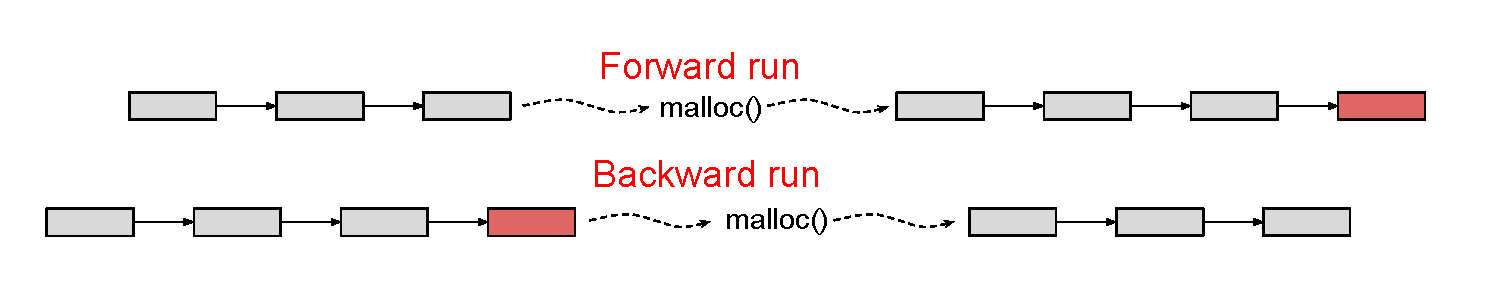
\includegraphics[scale=0.4]{ex/at.pdf}
			\end{center}
			\pause
			\item Reversion of \hlbl{abstraction} $\rightarrow$ \hlgr{intersection} of FA
			\begin{itemize}
				\item Consider FA $F_1=(TA_1^1,\ldots,TA_n^1)$ and $F_2=(TA_1^2,\ldots,TA_n^2)$,
					intersection is done \hlgr{component-wise} using TA intersection, i.e.,
					$F_1 \cap F_2 = (TA_1^1 \cap TA_1^2,\ldots,TA_n^1 \cap TA_n^2)$
			\end{itemize}
		\end{itemize}
		\pause
		\item \hlgr{Ingredients for predicate languages abstraction}:
		\begin{itemize}
			\item Predicates represented by TA
			\item Perform intersection of each TA of FA with all predicate automata
			\item Obtain a labelling of FA states by predicate automata states
			\item Collapses the states with the same labelling
		\end{itemize}
	\end{itemize}

\end{frame}

%*******************************************************************************

%*******************************************************************************
\begin{frame}
\frametitle{Boxes}

\begin{itemize}
		\item We use \hlbl{boxes} to extend expressive power of FA
		\item A box is a FA that can be used as a symbol of another FA
		\item A box represents repeating subgraphs of a heap
		\item FA having boxes in alphabet are called \hlbl{hierarchical}
	\end{itemize}
		\vspace{-0.8cm}
		\centering \usetikzlibrary{calc,matrix,backgrounds,fit,shapes,arrows}
\begin{tikzpicture}[
  scale=1.0,
  transform shape,
  node distance=18mm
]

  \path[use as bounding box] (-8mm,-3mm) rectangle (93mm,18mm);

  \tikzstyle{memnode}=[draw,rectangle,fill=lightgray,thick,minimum height=4.5mm, minimum width=4.5mm,inner sep=1mm,node distance=18mm,font=\tt]
  \tikzstyle{memnodeblue}=[draw,rectangle,fill=blue!30,thick,minimum height=4.5mm, minimum width=4.5mm,inner sep=1mm,node distance=18mm,font=\tt]
  \tikzstyle{memnodepink}=[draw,rectangle,fill=red!30,thick,minimum height=4.5mm, minimum width=4.5mm,inner sep=1mm,node distance=18mm,font=\tt]
  \tikzstyle{memnodegreen}=[draw,rectangle,fill=green!60,thick,minimum height=4.5mm, minimum width=4.5mm,inner sep=1mm,node distance=18mm,font=\tt]
  \tikzstyle{memnodepurple}=[draw,rectangle,fill=purple!60,thick,minimum height=4.5mm, minimum width=4.5mm,inner sep=1mm,node distance=18mm,font=\tt]
  \tikzstyle{memnodeorange}=[draw,rectangle,fill=orange!60,thick,minimum height=4.5mm, minimum width=4.5mm,inner sep=1mm,node distance=18mm,font=\tt]



  \tikzstyle{nullnode}=[node distance=18mm,label=center:$\bot$]
  \tikzstyle{varnode}=[font=\tt]
  \tikzstyle{refnode}=[fill=lightgray!40,minimum height=4.5mm, minimum width=4.5mm,inner sep=1mm,font=\tt]

  \tikzstyle{pointer}=[draw,->,>=latex,bend left]
  \tikzstyle{ptrlab}=[above,font=\tt]
  \tikzstyle{nextptr}=[label={[label distance=0mm,font=\tt]90:next}]
  \tikzstyle{prevptr}=[label={[label distance=0mm,font=\tt]-90:prev}]


  % nodes
  \node[memnodepink] (x1) at (0mm,0mm) {1};
  \node[memnodeblue] (x2) [right of=x1] {2};
  \node[memnodegreen] (x3) [right of=x2] {3};
  \node[memnodepurple] (x4) [right of=x3] {4};
  \node[memnodeorange] (x5) [right of=x4] {5};

%  \node[nullnode] (x5null) [right of=x5] {};
  \node (x5null) [right of=x5] {\dots};

  \node[varnode,node distance=5mm] (x) [left of=x1] {x:};

  % pointers
  \draw[pointer] (x1)    edge node[nextptr]   {} (x2);
  \draw[pointer] (x2)    edge node[nextptr]   {} (x3);
  \draw[pointer] (x3)    edge node[nextptr]   {} (x4);
  \draw[pointer] (x4)    edge node[nextptr]   {} (x5);
  \draw[pointer] (x5)    edge node[nextptr]   {} (x5null);


  \draw[pointer] (x2)    edge node[prevptr]   {} (x1);
  \draw[pointer] (x3)    edge node[prevptr]   {} (x2);
  \draw[pointer] (x4)    edge node[prevptr]   {} (x3);
  \draw[pointer] (x5)    edge node[prevptr]   {} (x4);
  \draw[pointer] (x5null)    edge node[prevptr]   {} (x5);

\end{tikzpicture}
\\
		\vspace{0.7cm}
		\centering DLS $=$ \usetikzlibrary{calc,matrix,backgrounds,fit,shapes,arrows}
\begin{tikzpicture}[
  scale=0.8,
  transform shape,
  node distance=18mm,
  anchor=base,
  baseline
]

  \tikzstyle{memnode}=[draw,rectangle,fill=lightgray,thick,minimum height=4.5mm, minimum width=4.5mm,inner sep=1mm,node distance=18mm,font=\tt]
  \tikzstyle{memnodeblue}=[draw,rectangle,fill=blue!30,thick,minimum height=4.5mm, minimum width=4.5mm,inner sep=1mm,node distance=18mm,font=\tt]
  \tikzstyle{memnodepink}=[draw,rectangle,fill=red!30,thick,minimum height=4.5mm, minimum width=4.5mm,inner sep=1mm,node distance=18mm,font=\tt]
  \tikzstyle{memnodegreen}=[draw,rectangle,fill=green!60,thick,minimum height=4.5mm, minimum width=4.5mm,inner sep=1mm,node distance=18mm,font=\tt]
  \tikzstyle{memnodepurple}=[draw,rectangle,fill=purple!60,thick,minimum height=4.5mm, minimum width=4.5mm,inner sep=1mm,node distance=18mm,font=\tt]
  \tikzstyle{memnodeorange}=[draw,rectangle,fill=orange!60,thick,minimum height=4.5mm, minimum width=4.5mm,inner sep=1mm,node distance=18mm,font=\tt]



  \tikzstyle{nullnode}=[node distance=18mm,label=center:$\bot$]
  \tikzstyle{varnode}=[font=\tt]
  \tikzstyle{refnode}=[fill=lightgray!40,minimum height=4.5mm, minimum width=4.5mm,inner sep=1mm,font=\tt]

  \tikzstyle{pointer}=[draw,->,>=latex,bend left]
  \tikzstyle{ptrlab}=[above,font=\tt]
  \tikzstyle{nextptr}=[label={[label distance=0mm,font=\tt]90:next}]
  \tikzstyle{prevptr}=[label={[label distance=0mm,font=\tt]-90:prev}]


  % nodes
  \node[memnodegreen] (x1) at (0mm,0mm) {1};
  \node[memnodepink] (x2) [right of=x1] {2};

  \node[above of=x1,yshift=-14.3mm,black!50] {\scriptsize in};
  \node[above of=x2,yshift=-14.3mm,black!50] {\scriptsize out};


  % pointers
  \draw[pointer] (x1)    edge node[nextptr]   {} (x2);

  \draw[pointer] (x2)    edge node[prevptr]   {} (x1);

\end{tikzpicture}
\\
		\vspace{-0.8cm}
		\centering \usetikzlibrary{calc,matrix,backgrounds,fit,shapes,arrows}
\begin{tikzpicture}[
  scale=0.8,
  transform shape,
  node distance=18mm
]

  \path[use as bounding box] (-8mm,-4mm) rectangle (93mm,18mm);

  \tikzstyle{memnode}=[draw,circle,thick,minimum height=4.5mm, minimum width=4.5mm,inner sep=1mm,node distance=18mm,font=\tt]
  \tikzstyle{memnodeblue}=[draw,rectangle,fill=blue!30,thick,minimum height=4.5mm, minimum width=4.5mm,inner sep=1mm,node distance=18mm,font=\tt]
  \tikzstyle{memnodepink}=[draw,rectangle,fill=red!30,thick,minimum height=4.5mm, minimum width=4.5mm,inner sep=1mm,node distance=18mm,font=\tt]
  \tikzstyle{memnodegreen}=[draw,rectangle,fill=green!60,thick,minimum height=4.5mm, minimum width=4.5mm,inner sep=1mm,node distance=18mm,font=\tt]

  \tikzstyle{nullnode}=[node distance=18mm,label=center:$\bot$]
  \tikzstyle{varnode}=[font=\tt]
  \tikzstyle{refnode}=[fill=lightgray!40,minimum height=4.5mm, minimum width=4.5mm,inner sep=1mm,font=\tt]

  \tikzstyle{pointer}=[draw,->,>=latex]
  \tikzstyle{ptrlab}=[above,font=\tt]
  \tikzstyle{nextptr}=[label={[draw,fill=blue!30,label distance=1mm]90:DLS }]
  \tikzstyle{prevptr}=[label={[label distance=0mm,font=\tt]-90:prev}]


  % nodes
  \node[memnode] (x1) at (0mm,0mm) {$q_1$};
  \node[memnode] (x2) [right of=x1] {$q_2$};
  \node[memnode] (x3) [right of=x2] {$q_3$};
  \node[memnode] (x4) [right of=x3] {$q_4$};
  \node[memnode] (x5) [right of=x4] {$q_5$};

%  \node[nullnode] (x5null) [right of=x5] {};
  \node (x5null) [right of=x5] {\dots};

%  \node[varnode,node distance=5mm] (x) [left of=x1] {x:};

  % pointers
  \draw[pointer] (x1)    edge node[nextptr]   {} (x2);
  \draw[pointer] (x2)    edge node[nextptr]   {} (x3);
  \draw[pointer] (x3)    edge node[nextptr]   {} (x4);
  \draw[pointer] (x4)    edge node[nextptr]   {} (x5);
  \draw[pointer] (x5)    edge node[nextptr]   {} (x5null);

\end{tikzpicture}

\end{frame}

%*******************************************************************************


%*******************************************************************************
\begin{frame}
\frametitle{Backward run with Hierarchical Forest Automata}
	
		   	\begin{itemize}
				\item To enable component-wise hierarchical FA intersection,
					so called \hlbl{compatible form} of FA is needed:
				\begin{itemize}
					\item They have same number of TA
					\item \hlbl{The same subgraphs are folded into the same boxes}
				\end{itemize}
				\item Compatible form is preserved during backward run
			\end{itemize}

	\begin{center}
		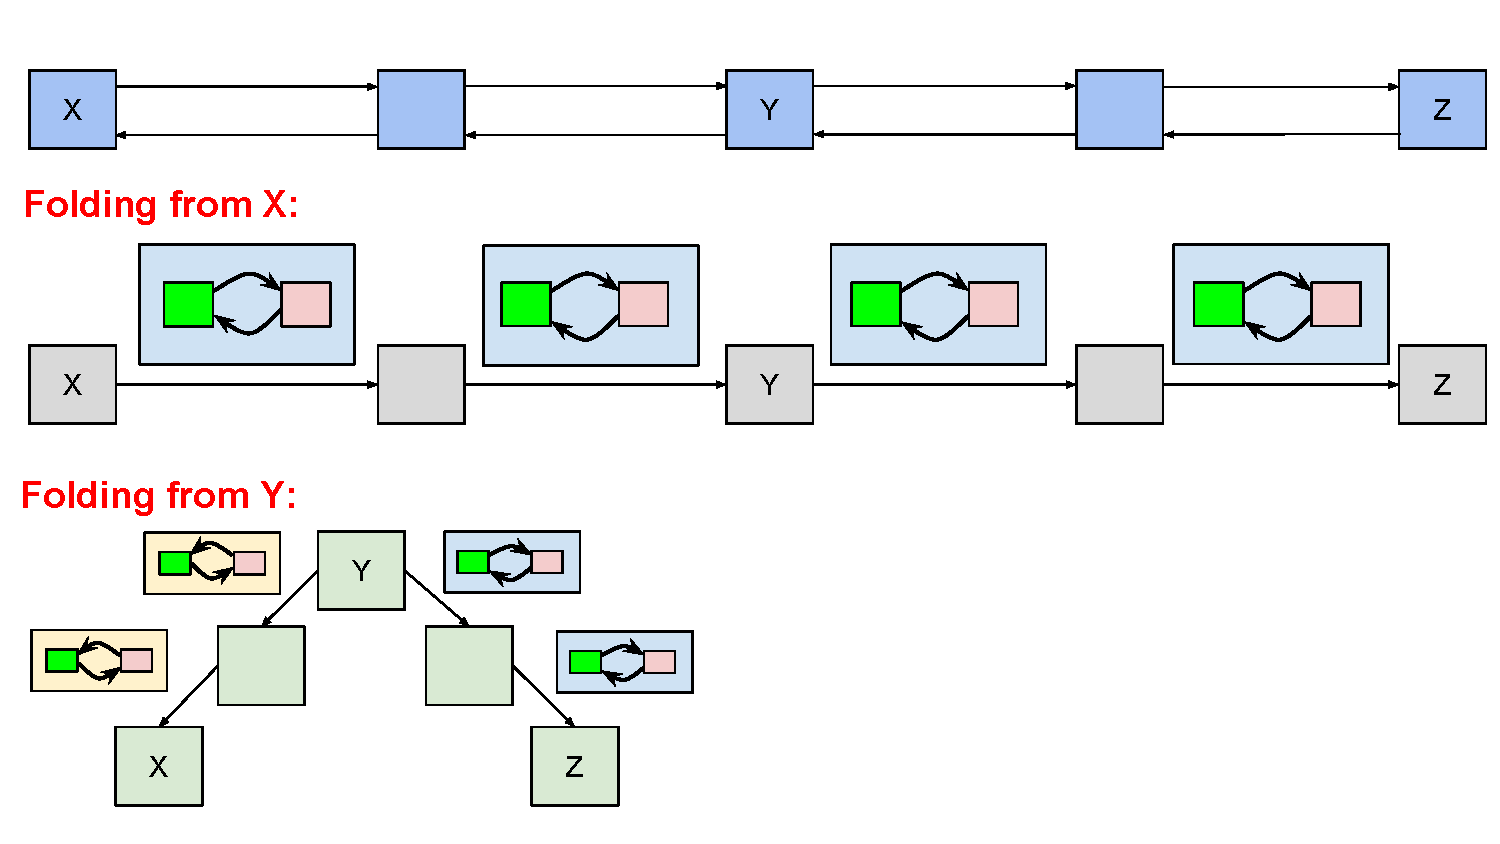
\includegraphics[scale=0.4]{ex/cp.pdf}
	\end{center}

\end{frame}
%*******************************************************************************


%*******************************************************************************
\begin{frame}
\frametitle{Intersection with Hierarchical Forest Automata}

  	\begin{itemize}
	\item \hlbl{Intersection of FA} is done:
		  	\begin{itemize}
				\item Component-wise using TA intersection
				\item When TA intersection reaches boxes in the transitions of both automata it calls the whole
					procedure for \hlbl{FA intersection recursively on the boxes} and uses its results as a new box
			\end{itemize}
	\end{itemize}
	\begin{center}
		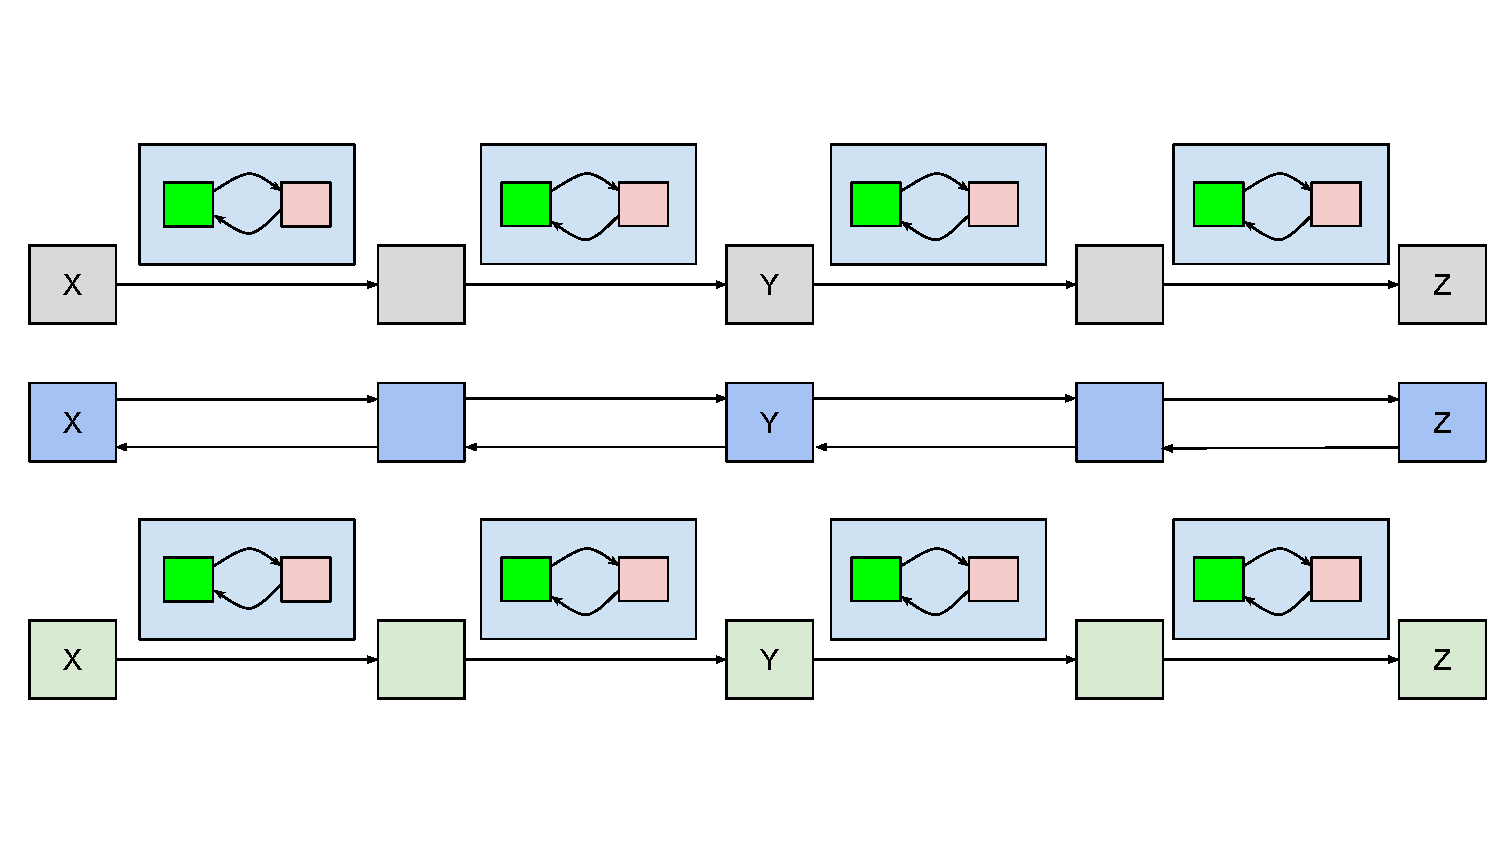
\includegraphics[scale=0.4]{ex/is.pdf}
	\end{center}

\end{frame}
%*******************************************************************************

%*******************************************************************************
\begin{frame}
\frametitle{Experimental Evaluation}

	\begin{center}
	\begin{adjustbox}{max height=\textheight, max width=\textwidth}
	%\tiny
	%\caption{Results of experiments.}
	\begin{tabular}{| l | l | r | r | r | r || l | l | r | r | r | r | r |}
        \hline
		Program & Status & LoC & Time [s] & Refnm& Preds & Program & Status & LoC & Time [s] & Refnm & Preds \\
        \hline
        \hline
		SLL (delete) & \cellcolor{\scol{}} \safe & $33$ & $0.02$ &  $0$ & $0$ & DLL (rev) & \cellcolor{\scol{}} \safe & $39$ &  $0.70$ & $0$  & $0$ \\
        \hline
		SLL (bubblesort) & \cellcolor{\scol{}} \safe & $42$ & $0.02$ &  $0$ & $0$ & CDLL & \cellcolor{\scol{}} \safe & $32$ &  $0.02$  & $0$  & $0$ \\
        \hline
		SLL (insertsort) & \cellcolor{\scol{}} \safe & $36$ & $0.04$ & $0$ & $0$ & DLL (insertsort) & \cellcolor{\scol{}} \safe & $42$ &  $0.56$  & $0$  & $0$ \\
        \hline
		SLLOfCSLL & \cellcolor{\scol{}} \safe & $47$ & $0.02$ & $0$ & $0$ & DLLOfCDLL & \cellcolor{\scol{}} \safe & $54$ &  $1.76$  & $0$  & $0$ \\
        \hline
		\rowcolor{\hcol{}}
		\textbf{SLL01}    & \cellcolor{\scol{}} \safe & $70$ & $1.20$   &  $1$ & $1$ & \textbf{DLL01} & \cellcolor{\scol{}} \safe & $73$ &  $0.65$  & $2$  & $2$ \\
        \hline
		\rowcolor{\hcol{}}
		\textbf{CircularSLL} & \cellcolor{\scol{}} \safe & $49$ & $3.57$   &  $3$  & $3$ & \textbf{CircularDLL} & \cellcolor{\scol{}} \safe  & $52$ &  $37.22$ & $18$ & $24$ \\
        \hline
		\rowcolor{\hcol{}}
		\textbf{OptPtrSLL}   & \cellcolor{\scol{}} \safe & $59$ & $1.90$ & $3$ & $3$ & \textbf{OptPtrDLL} &\cellcolor{\scol{}} \safe & $62$ &  $1.87$  & $5$ & $5$ \\
        \hline
		\rowcolor{\hcol{}}
		\textbf{QueueSLL}    & \cellcolor{\scol{}} \safe & $71$ & $11.32$  &  $10$ & $10$ & \textbf{QueueDLL} &  \cellcolor{\scol{}}  \safe  & $74$ &  $44.68$ & $14$ & $14$ \\
		\rowcolor{\hcol{}}
        \hline
		\textbf{GBSLL}       & \cellcolor{\scol{}} \safe & $64$ & $0.84$   &  $3$ & $3$ & \textbf{GBDLL} &  \cellcolor{\scol{}}  \safe & $71$ &  $1.89$  & $4$ & $4$ \\
        \hline
		\rowcolor{\hcol{}}
		\textbf{GBSLLSent}   & \cellcolor{\scol{}} \safe  & $68$ & $0.85$   &  $3$ & $3$ & \textbf{GBDLLSent} & \cellcolor{\scol{}} \safe & $75$ &  $2.19$  & $4$ & $4$ \\
        \hline
		\rowcolor{\hcol{}}
		\textbf{RGSLL}       & \cellcolor{\scol{}} \safe & $72$ & $14.41$  &  $22$  & $38$ & \textbf{RGDLL} & \cellcolor{\scol{}} \safe & $76$ &  $78.76$ & $26$ & $26$ \\
        \hline
		\rowcolor{\hcol{}}
		\textbf{WBSLL}       & \cellcolor{\scol{}} \safe & $62$ & $0.84$   &  $5$  & $5$ & \textbf{WBDLL} & \cellcolor{\scol{}} \safe & $71$ &  $1.37$  & $7$ & $7$ \\
        \hline
		\rowcolor{\hcol{}}
		\textbf{SortedSLL}   & \cellcolor{\scol{}} \safe & $76$ & $227.12$ &  $15$ & $15$ & \textbf{SortedDLL} & \cellcolor{\scol{}} \safe & $82$ &  $36.67$ & $11$ & $11$ \\
        \hline
		\rowcolor{\hcol{}}
		\textbf{EndSLL}      & \cellcolor{\scol{}} \safe  & $45$ & $0.07$   &  $2$  & $2$ & \textbf{EndDLL} & \cellcolor{\scol{}} \safe & $49$ &  $0.10$  & $3$ & $3$ \\
        \hline
		\rowcolor{\hcol{}}
		\textbf{TreeRB} & \cellcolor{\ucol{}}\unsafe & $130$ &  $0.08$  & $0$  & $0$ & \textbf{TreeWB} & \cellcolor{\ucol{}}\unsafe & $125$ &  $0.05$  & $0$ & $0$ \\
        \hline
		TreeCnstr & \cellcolor{\scol{}} \safe & $52$ & $0.31$  & $0$  & $0$ & \cellcolor{\hcol{}}\textbf{TreeCnstr} & \cellcolor{\ucol{}}\unsafe & \cellcolor{\hcol{}} $52$ & \cellcolor{\hcol{}} $0.03$  & \cellcolor{\hcol{}} $0$ & \cellcolor{\hcol{}} $0$ \\
        \hline
		TreeOfCSLL & \cellcolor{\scol{}} \safe & $109$ &  $0.57$  & $0$  & $0$ & \cellcolor{\hcol{}}\textbf{TreeOfCSLL}  & \cellcolor{\ucol{}}\unsafe & \cellcolor{\hcol{}} $109$ & \cellcolor{\hcol{}} $0.56$  & \cellcolor{\hcol{}} $1$ & \cellcolor{\hcol{}} $3$ \\
        \hline
		TreeStack & \cellcolor{\scol{}} \safe & $58$ &  $0.20$  & $0$  & $0$ & \cellcolor{\hcol{}}\textbf{TreeStack} & \cellcolor{\ucol{}}\unsafe & \cellcolor{\hcol{}} $58$ & \cellcolor{\hcol{}} $0.01$  & \cellcolor{\hcol{}} $0$ & \cellcolor{\hcol{}} $0$ \\
        \hline
		TreeDSW   & \cellcolor{\scol{}} \safe & $72$ & $1.87$  & $0$  & $0$ & \cellcolor{\hcol{}}\textbf{TreeDSW} & \cellcolor{\ucol{}}\unsafe & \cellcolor{\hcol{}} $72$ & \cellcolor{\hcol{}} $0.02$  & \cellcolor{\hcol{}} $0$ &  \cellcolor{\hcol{}} $0$ \\
		\hline
		TreeRootPtr & \cellcolor{\scol{}} \safe & $62$ &  $1.43$  & $0$  &  $0$ & \cellcolor{\hcol{}}\textbf{TreeRootPtr} & \cellcolor{\ucol{}}\unsafe & \cellcolor{\hcol{}} $62$ & \cellcolor{\hcol{}} $0.17$  & \cellcolor{\hcol{}} $2$ & \cellcolor{\hcol{}} $6$\\
        \hline
		SkipList    & \cellcolor{\scol{}} \safe & $84$ & $3.36$  & $0$  & $0$ & \cellcolor{\hcol{}}\textbf{SkipList} & \cellcolor{\ucol{}}\unsafe & $\cellcolor{\hcol{}} 84$ & \cellcolor{\hcol{}} $0.08$  & \cellcolor{\hcol{}} $1$  & \cellcolor{\hcol{}} $1$ \\
        \hline
		% SkipList-3nd    & $97$ & $0.17$  & $1$  & N & x & $1$ & & & & & & & \\
        % \hline
	\end{tabular}
	\label{tab:times}
	\end{adjustbox}	
  % \vspace{-4mm}
  % \vspace{-8mm}
%\end{table}
	\end{center}

\end{frame}
%*******************************************************************************

%*******************************************************************************

\begin{frame}
  \frametitle{Conclusions}

  \begin{itemize}
	  \item \hlgr{Contribution:}
		\begin{itemize}
			\item Backward run and predicate languages abstraction for FA based shape analysis 
			\item Compatible form and intersection of FA
			\item Enable analysis of data structures with relation between nodes
			\item Experimentally evaluated on number of test cases
		\end{itemize}
		\item \hlgr{Future work:}
			\begin{itemize}
				\item Find out reasons of state explosion on complicated tree structures
			\end{itemize}
  \end{itemize}
\end{frame}
%*******************************************************************************

\end{document}
